\documentclass[lettersize,journal]{IEEEtran}
\usepackage{amsmath,amsfonts}
\usepackage{algorithm}
\usepackage{algpseudocode}
\usepackage{amssymb}
\usepackage{array}
\usepackage[caption=false,font=normalsize,labelfont=sf,textfont=sf]{subfig}
\usepackage{textcomp}
\usepackage{stfloats}
\usepackage{url}
\usepackage{verbatim}
\usepackage{graphicx}
\usepackage{cite}
\usepackage{booktabs}
\algrenewcommand{\algorithmiccomment}[1]{\hfill$\triangleright$ #1}
\algrenewcommand\algorithmicrequire{\textbf{Input:}}
\algrenewcommand\algorithmicensure{\textbf{Output:}}
\hyphenation{op-tical net-works semi-conduc-tor IEEE-Xplore}
% updated with editorial comments 8/9/2021

\begin{document}

\title{A Vision-Driven Closed-Loop Framework  \\ for High-Precision Robotic Baggage Handling}



% The paper headers
\markboth{Journal of \LaTeX\ Class Files,~Vol.~14, No.~8, August~2021}%
{Shell \MakeLowercase{\textit{et al.}}: A Sample Article Using IEEEtran.cls for IEEE Journals}


% Remember, if you use this you must call \IEEEpubidadjcol in the second
% column for its text to clear the IEEEpubid mark.

\maketitle

\begin{abstract}
Robotic baggage handling in airport logistics requires not only reliable grasp execution but also accurate geometric alignment under high-throughput industrial constraints. Existing vision-based manipulation pipelines usually process perception, geometric modeling, and motion control as weakly coupled modules. As a result, their performance can degrade when baggage tags and straps introduce visual interference, when residual mask errors are amplified during 2D to 3D projection, or when conveyor motion causes temporally unstable observations. This paper presents a closed-loop perception--geometric modeling--control framework for dynamic robotic baggage handling. The proposed system improves 2D instance segmentation through multi-scale feature aggregation and attention-guided mask refinement, enhances 3D geometric reliability using pixel-to-3D cross-consistency filtering and temporal oriented bounding-box (OBB) stabilization, and performs predictive grasp execution through recursive state estimation, coarse-to-fine interception planning, and active state regulation. By tightly coupling semantic perception, spatio-temporal geometry refinement, and motion planning, the framework addresses the precision requirements of suction-based grasping and dense baggage arrangement in airport logistics. Experiments on a real robotic platform show that the general grasp success rate remains consistently high, increasing from 93.6\% to 96.4\%, while the precision success rate improves from 62.1\% to 92.7\%. These results indicate that the proposed framework primarily improves pose accuracy and placement reliability rather than merely increasing lift success, making it suitable for high-throughput and high-density baggage handling applications.
\end{abstract}

\renewcommand{\abstractname}{Note to Practitioners}
\begin{abstract}
This paper addresses the practical challenges of automating baggage handling in high-speed airport logistics. While industrial robotic arms are highly capable, they struggle to reliably grasp and densely pack baggage from moving conveyor belts. Baggage often features flexible, distracting attachments, such as identification tags and loose straps, which traditional vision systems mistakenly treat as solid grasping points. Furthermore, the conveyor's continuous motion causes tracking errors, leading to failed lifts or inaccurate placements.  To solve these issues, we introduce a tightly integrated framework connecting the robot's perception directly to its motion controls. First, tailored image processing accurately outlines the rigid baggage body while explicitly ignoring flexible tags. Second, the system builds a reliable 3D model by filtering depth-sensor noise and smoothing visual jitters. Finally, it predicts the moving baggage's future path, enabling the robotic arm to synchronize its speed and seamlessly intercept the target. If baggage is stacked in a confusing way, the robot actively rearranges items to improve visibility.  In real-world tests, this approach improved the precision of placement from 62.1\% to 92.7\%. This demonstrates that the framework achieves the high-accuracy positioning required to tightly pack baggage into containers. 
\end{abstract}

\begin{IEEEkeywords}
Robotic Baggage Handling, Industrial Robotics, Predictive Motion Planning, 3D Pose Estimation.
\end{IEEEkeywords}

\section{Introduction}
\IEEEPARstart{R}{obotic} baggage handling is becoming an important component of intelligent airport logistics, where sorting, loading, and transfer operations must be performed reliably within strict time windows. Vision feedback is essential in such systems because it connects object perception with grasp planning and execution. Classical visual servoing establishes closed-loop control by mapping visual feature errors to robot motion commands \cite{hutchinson2002tutorial}. However, in practical baggage handling environments, the dominant bottleneck is often not the control law itself, but the reliability and geometric fidelity of the visual observations used by the controller. Baggage items are visually heterogeneous, frequently occluded, and often equipped with deformable tags, straps, wheels, and handles. These factors make the perception-to-action pipeline substantially more difficult than standard pick-and-place manipulation with regular objects.

Conventional robotic grasping pipelines usually detect the target in RGB images and then fuse depth information for 6D pose or 3D bounding-box estimation. Bounding-box-based detection is efficient but lacks the boundary-level accuracy required for precise manipulation, especially when objects are stacked, partially occluded, or densely arranged. Instance segmentation improves spatial localization by separating objects at the pixel level, but segmentation errors at the boundary may still be amplified after projection into the point cloud. In baggage scenarios, flexible tags and straps are particularly problematic: they may be segmented as part of the rigid body in the image, but they do not belong to the stable geometric structure needed for grasping and placement.

Airport baggage handling further imposes several coupled challenges. First, visual interference arises from highly salient and deformable components such as identification tags, ropes, ribbons, and straps. General purpose segmentation models \cite{he2017mask} may regard these components either as independent objects or as part of the suitcase body, which shifts the estimated centroid and degrades grasp accuracy. Second, 3D projection distortion occurs when residual 2D mask leakage produces outliers in the projected point cloud. Such outliers can bias PCA-based pose estimation and OBB construction \cite{rusu20113d, gottschalk1996obbtree}. Third, temporal instability is caused by conveyor motion, sliding, rolling, collision-induced disturbances, motion blur, and depth-sensor noise. These factors introduce frame-to-frame jitter that directly affects predictive grasping. Finally, high-tempo industrial constraints require the robot to grasp moving targets within a short time window. In our system, the conveyor speed reaches approximately 0.5$\mathrm{m/s}$. Downstream loading also requires high space utilization, so even small pose errors or volume-estimation errors may reduce packing density and increase the number of required loading cycles.

Suction grasping is attractive for dense baggage scenes because it requires limited lateral insertion space, unlike a mechanical gripper that often needs side clearance. Nevertheless, suction grasping is sensitive to local surface localization and pose accuracy. A successful suction grasp therefore depends on reliable segmentation, stable 3D modeling, and accurate motion prediction \cite{bohg2013data}. In this work, a dedicated hybrid end-effector is designed that integrates both suction and a gripper mechanism. The gripper is used as the primary interaction mode for all luggage, while suction serves as a complementary capability for specific cases where it is advantageous. This hardware configuration motivates a closed-loop software architecture in which perception, geometric modeling, and control are optimized jointly rather than treated as isolated modules.

To address the above issues, this paper proposes a vision-driven closed-loop perception, geometric modeling and control framework for high-precision robotic baggage handling. At the perception level, a Multi-Scale Feature Aggregation and Attention-Guided Mask Optimization Network (MSAM-Net) is developed to obtain accurate instance masks under tag and strap interference. At the geometric modeling level, a pixel-to-3D Cross Consistency Conditional Filtering (PX3C) method removes residual flexible outliers after 2D-to-3D projection, and a Consistency-Aware OBB Stabilization (CAOS) strategy enforces temporal smoothness across frames. At the action level, a discrete Kalman-filter-based recursive Bayesian estimator predicts target states, a two-stage relative-velocity planning strategy executes rapid interception followed by precise synchronization, and an active state-regulation mechanism resets highly uncertain baggage configurations when passive observation is unreliable.

The contributions of this paper are summarized as follows.
\begin{itemize}
  \item A real-time semantic perception network, MSAM-Net, is proposed for baggage instance segmentation under severe visual interference. The network combines four-level multi-branch feature aggregation with attention-guided multi-scale mask refinement.
  \item A spatio-temporal geometric modeling framework is introduced. PX3C removes residual 3D interference by enforcing pixel-to-3D geometric consistency, and CAOS stabilizes OBB pose and scale estimates using quality-aware temporal smoothing.
  \item A closed-loop dynamic grasping strategy is developed by integrating recursive Bayesian state estimation, two-stage relative-velocity planning, and active state regulation. The complete system is validated on a real robotic baggage-handling platform.
\end{itemize}
\section{Related Works}
\subsection{Visual Servoing for Robotic Manipulation}
Visual servoing is a closed-loop control paradigm in which visual measurements are used to reduce the error between the current and desired robot states \cite{chaumette2008visual}, and has been widely used in robotics \cite{wang2023visual, he2023image}. Depending on the error space, visual servoing is usually categorized into image-based visual servoing (IBVS) and position-based visual servoing (PBVS) . IBVS defines the control error directly in the image plane and can avoid explicit 3D reconstruction in some tasks, but it may suffer from depth ambiguity, image-Jacobian singularity, and complex camera-motion coupling. PBVS \cite{lippiello2007position} defines the error in 3D Cartesian space and therefore supports explicit trajectory planning, which is useful for industrial manipulation. However, PBVS requires reliable 3D pose estimation \cite{zhu2024position, chaumette2008visual}. In unstructured baggage handling, this requirement becomes the main limitation because visual observations are noisy, dynamic, and affected by flexible attachments. Therefore, a robust perception and geometric modeling frontend is a prerequisite for stable PBVS-style manipulation in this work.

\subsection{Object Detection and Instance Segmentation}
Accurate object perception is the foundation of robotic manipulation. Traditional 2D detectors such as Faster R-CNN \cite{ren2015faster} and 3D detectors such as PointNet++ \cite{qi2017pointnet++} and PV-RCNN \cite{shi2020pv} primarily output bounding boxes. Although bounding boxes are computationally efficient, they provide only coarse geometric support and can introduce significant extrapolation errors when baggage items overlap or touch each other. Instance segmentation methods, including Mask R-CNN \cite{he2017mask}, YOLACT \cite{bolya2019yolact}, and YOLO-based segmentation models \cite{Jocher_Ultralytics_YOLO26_Unified_2026}, provide pixel-level object separation and are therefore more suitable for downstream point-cloud extraction. Foundation models such as Segment Anything Model (SAM) \cite{kirillov2023segment} show strong generalization, but their computational cost is usually too high for embedded real-time robotic control. In this paper, a lightweight YOLOv10-based architecture is modified for baggage segmentation so that real-time inference can be maintained while the specific tag-interference problem is addressed.

\subsection{3D Geometric Modeling and Point-Cloud Refinement}

After obtaining the 2D target mask, robotic grasping requires accurate 3D geometric modeling to estimate the object pose and dimensions. Classical pipelines usually rely on the Point Cloud Library (PCL) \cite{rusu20113d}, which provides standard operations such as VoxelGrid downsampling, statistical outlier removal, and RANSAC-based plane segmentation \cite{fischler1981random}. The cleaned point cloud is then commonly processed by Principal Component Analysis (PCA) to estimate the principal axes and construct an oriented bounding box (OBB). However, baggage-handling scenarios introduce several adverse sensing conditions. Reflective stickers, luggage tags, flexible straps, and conveyor motion may produce holes, ghost points, and local geometric distortions in depth observations from ToF or structured-light cameras. Therefore, depth completion and point cloud denoising have become important techniques for robust 3D geometric modeling.

Depth completion methods aim to recover missing geometry from incomplete depth measurements. For example, HDCNet \cite{xie2025hdcnet} adopts a hybrid architecture combining CNN, Transformer, and Mamba modules to infer the geometry of transparent or reflective objects from RGB and depth cues. Such methods can compensate for missing depths caused by specular reflection and reduce hole-induced pose errors. Nevertheless, they typically require large-scale training data and introduce considerable computational overhead. In baggage handling, reflective regions often appear only locally, such as on stickers or tags, while the main suitcase body is usually close to a regular cuboid. Therefore, a lightweight heuristic treatment is more suitable for real-time deployment.

Point cloud denoising has also been widely studied. Traditional filters, such as bilateral filtering \cite{digne2017bilateral, si2022lbf}, can suppress isolated outliers but are less effective for flexible accessories whose geometry does not follow smooth rigid surfaces. Graph-based methods further exploit local geometric similarity, such as feature graph learning with Graph Laplacian regularization \cite{hu2020feature}. However, these methods still rely heavily on local surface consistency assumptions, which may fail for thin tags and deformable straps. Recent learning-based denoising methods, including Total Denoising \cite{hermosilla2019total, rakotosaona2020pointcleannet}, and EC-Net \cite{yu2018ec}, improve general denoising performance but are not specifically designed for structured baggage accessories and often require additional computation.

Dynamic point cloud denoising further considers temporal inconsistency caused by object or sensor motion. Xu et al. proposed to use spatio-temporal convolution to aggregate gradient fields across frames \cite{hu2025dynamic}, while Hu et al. exploited intra-frame self-similarity and inter-frame consistency through spatio-temporal graph learning \cite{hu2021dynamic}. These approaches are effective for general dynamic point clouds, but they are usually designed for sensor motion or high-speed targets. In our setting, the camera is fixed and the conveyor speed is controllable. Therefore, instead of employing a heavy dynamic denoising network, this work introduces a task-specific Pixel-to-3D Cross Consistency Conditional Filtering (PX3C) module to remove flexible tags and straps, and a Consistency-Aware OBB Stabilization (CAOS) module to suppress frame-to-frame pose jitter. This design preserves the efficiency of classical PCL-based processing while improving robustness in practical baggage-grasping scenarios.


\subsection{Dynamic Grasping and Active Perception}

Grasp planning can be broadly categorized into static and dynamic approaches. Static grasp synthesis assumes that the target object remains stationary during perception and execution, and has been extensively studied in data-driven grasping literature \cite{bohg2013data}. However, this assumption is not suitable for conveyor-based baggage handling, where objects continuously move, collide, and may undergo pose changes during robot execution. Therefore, robust state estimation and time-aware motion planning are essential for dynamic grasping.

For moving target tracking, recursive Bayesian filtering provides a standard and efficient framework. Learning-based trajectory prediction methods, such as Social LSTM \cite{alahi2016social}, can model complex nonlinear motions, but they usually require large-scale training data and are unnecessary when the target motion is physically constrained. In conveyor scenarios, baggage motion is mainly governed by belt velocity with moderate sensing noise. Thus, a discrete Kalman filter with a constant-acceleration motion model \cite{li2003survey} offers a favorable trade-off between robustness and computational efficiency. For dynamic interception, Cowley et al. proposed a perception-and-planning framework for picking moving objects \cite{cowley2013perception}. Inspired by this idea, we adopt a two-stage hierarchical strategy that decouples fast global interception in Cartesian space from local synchronization in relative velocity space, thereby balancing execution speed and grasping precision.

Another limitation of many existing grasping systems is their reliance on passive perception. When the target enters a chaotic or high-uncertainty state, such as unstable stacking or severe occlusion, passive state estimation may become unreliable. Interactive perception has shown that robot actions can actively reveal occluded geometry and improve perception reliability \cite{bohg2017interactive}. Related studies on robotic rearrangement further aim to reorganize cluttered scenes to facilitate downstream manipulation \cite{batra2020rearrangement}. For example, DexSinGrasp \cite{xu2025dexsingrasp} and OPG-Policy \cite{ding2024opg} use dexterous hands or end-effectors to separate the target from surrounding clutter during grasping. Murray et al. further proposed an interactive visual failure prediction strategy, where probing actions such as lifting or shaking are used before grasp execution \cite{murray2024learning}. Although these methods mainly focus on static tabletop scenes, they motivate our active intervention strategy for conveyor-based grasping. Instead of simply stopping and retrying after failure, our system actively resets unstable target states and reduces scene uncertainty in real time.

Recently, Vision-Language-Action (VLA) models have attracted increasing attention in embodied AI by unifying perception, language understanding, and action generation. Representative examples include RT-2 \cite{zitkovich2023rt}, the Physical Intelligence $\pi$ series \cite{black2024pi_0, intelligence2025vision}, and OpenVLA \cite{kim2024openvla}. These models demonstrate strong potential in semantic reasoning and cross-task generalization. However, they typically involve billions of parameters, require large-scale training data, and often have limited inference frequency, which makes them difficult to deploy in high-speed industrial scenarios with strict real-time constraints. Therefore, for the conveyor-based grasping problem addressed in this work, we prioritize a lightweight model-based planning framework that provides predictable latency, explicit state estimation, and reliable real-time control.

\section{System Overview and Problem Formulation}
\subsection{System Architecture}
The proposed system forms a closed-loop perception, geometric modeling and control pipeline, as illustrated in Fig.~\ref{fig:overview}. The input consists of RGB-D images captured above the conveyor. The semantic perception module first segments baggage instances and suppresses tag-like visual interference. The geometric consistency module projects the selected mask into a point cloud, removes residual 3D outliers, and estimates a temporally stable OBB. The dynamic control module then predicts the target state, plans a coarse-to-fine interception trajectory, and executes grasping. If the uncertainty of the target state becomes too high, the active state-regulation module triggers a reset behavior.

\begin{figure*}[!t]
\centering
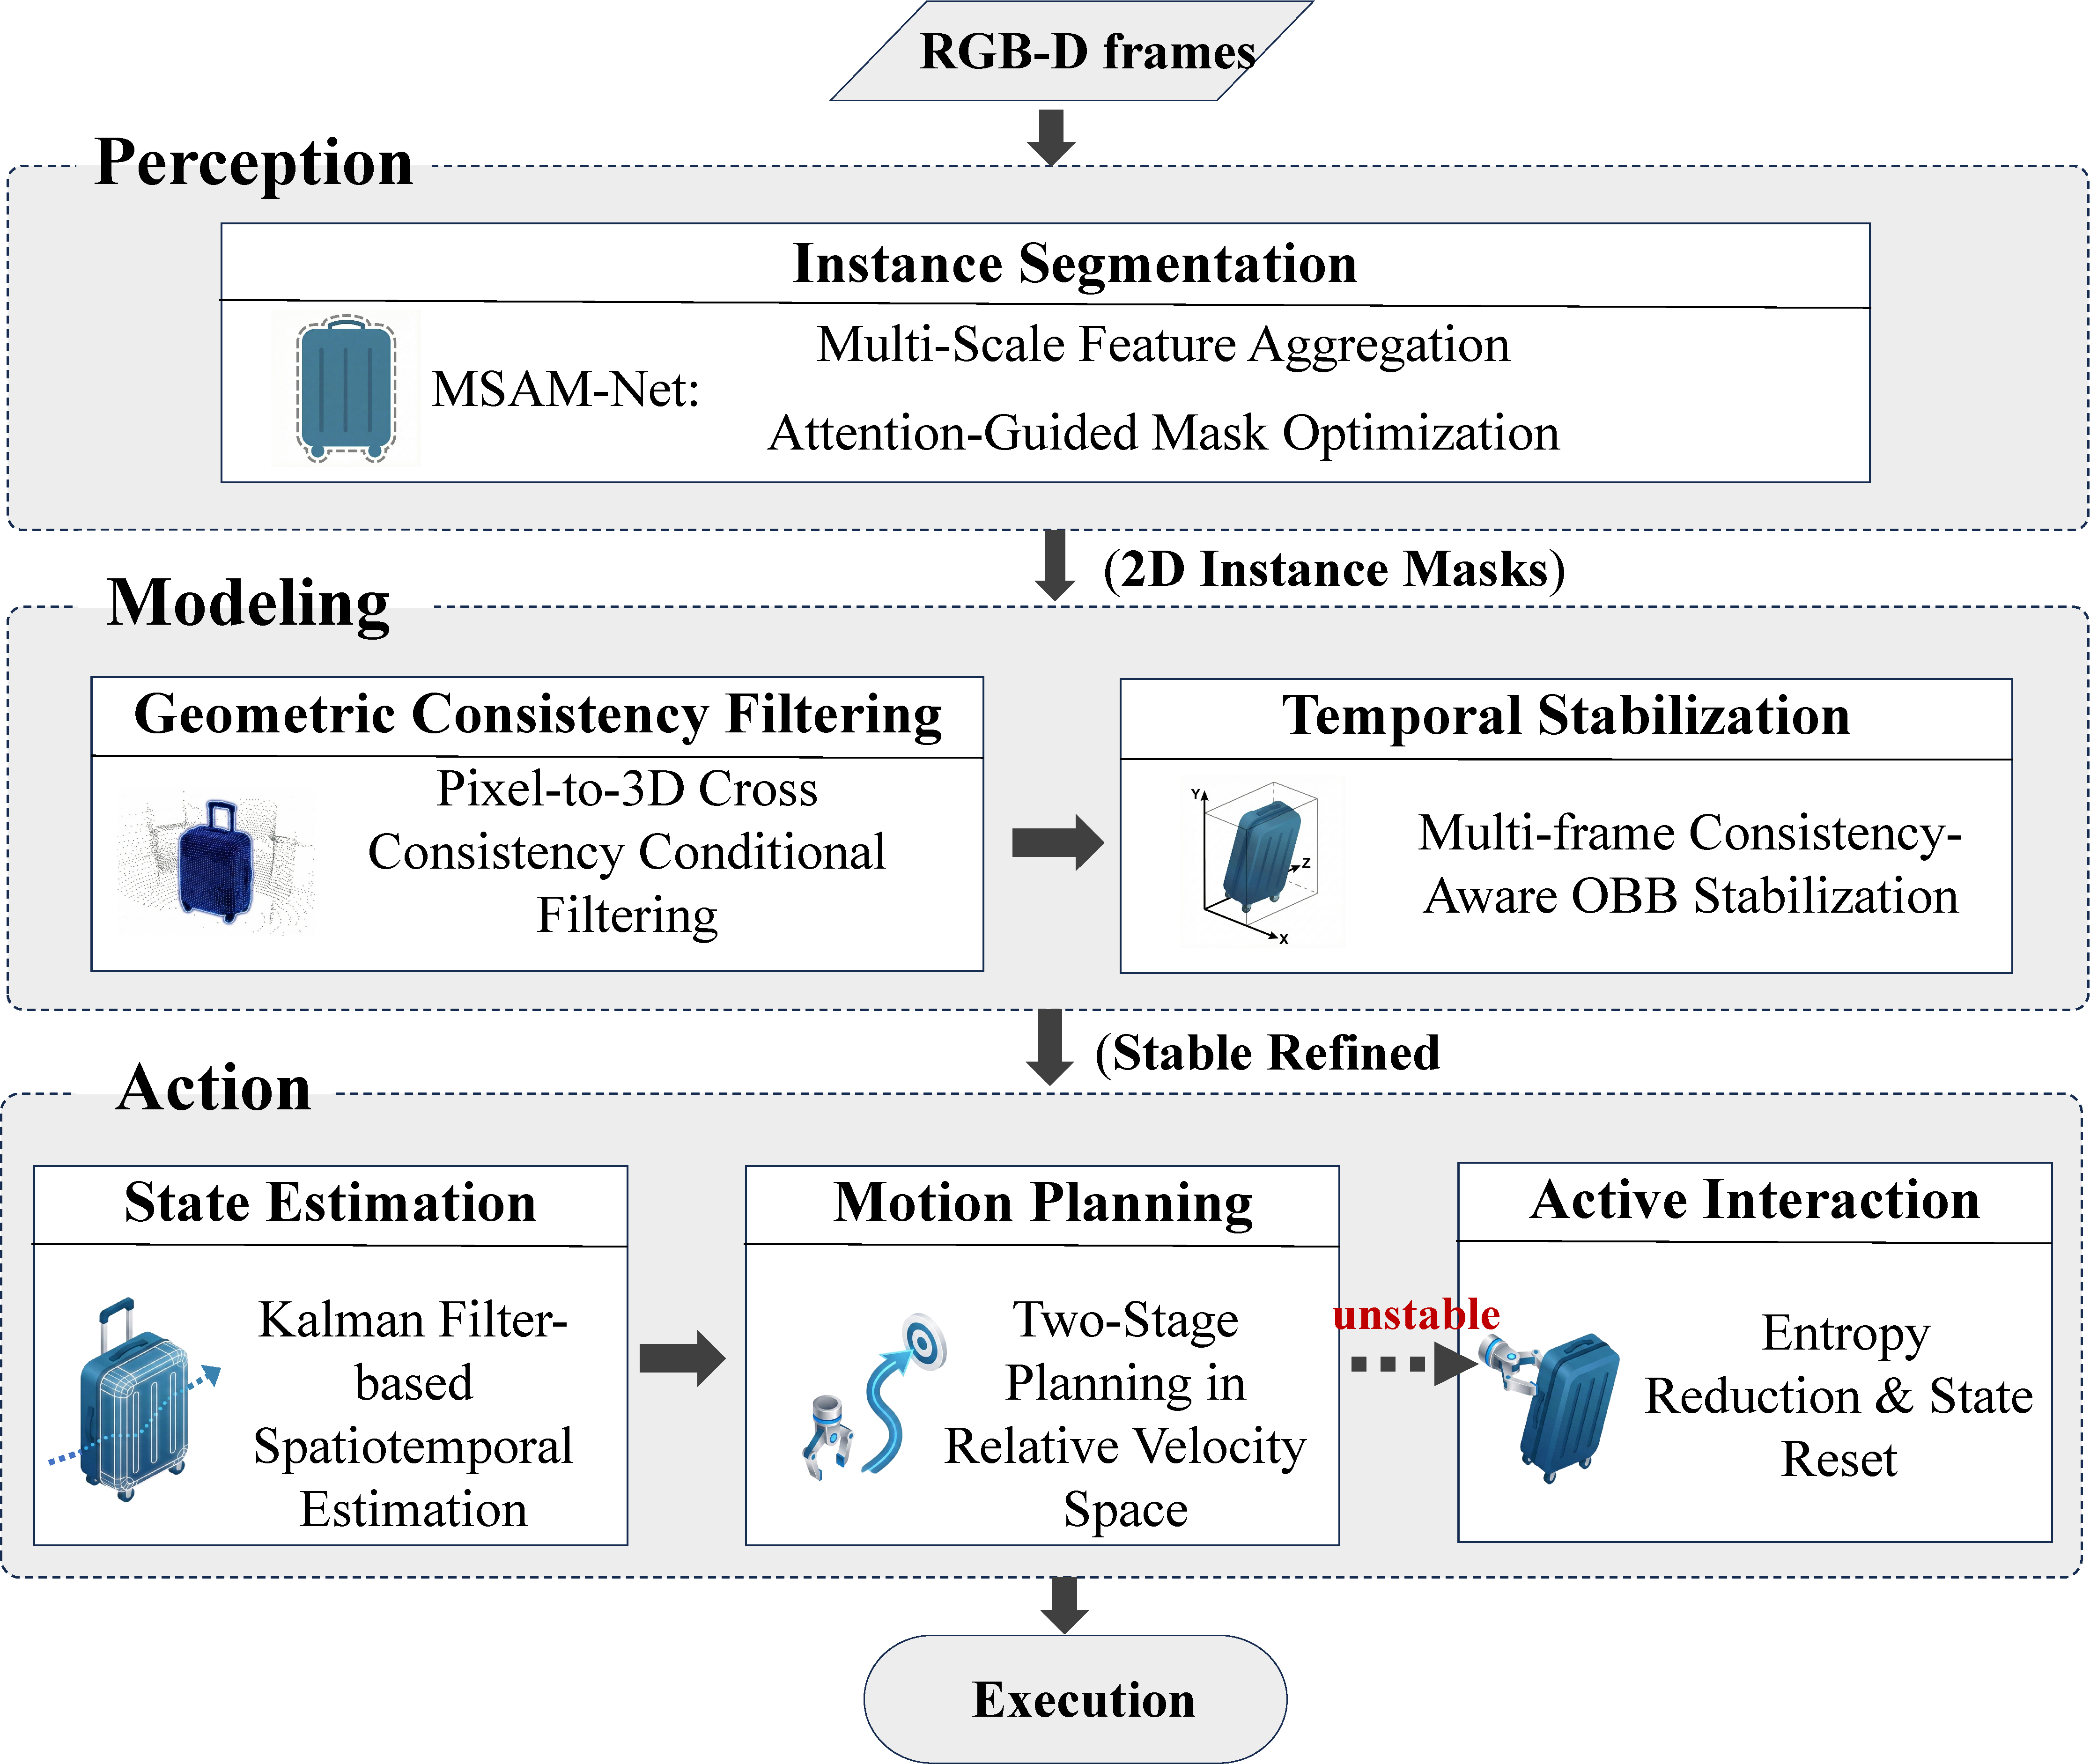
\includegraphics[width=\textwidth]{figures/fig1.pdf}
\caption{Overall framework of the proposed closed-loop perception, geometric modeling, and control system. RGB-D frames are first processed through instance segmentation (MSAM-Net) for mask refinement. The resulting point clouds undergo geometric consistency filtering (PX3C) and temporal stabilization (CAOS) to produce a reliable 3D representation. State estimation uses a Kalman-filter-based spatiotemporal approach, followed by two-stage motion planning in relative velocity space. Active interaction reduces environmental entropy and resets unstable object states, enabling robust real-time execution.}
\label{fig:overview}
\end{figure*}

The central design principle is to avoid irreversible error propagation. A segmentation error can create 3D outliers, a distorted OBB can produce an incorrect grasp pose, and an inaccurate pose can further cause poor placement. Therefore, each stage is designed to evaluate and refine the information passed to the next stage. The framework also closes the loop at the physical level: when passive perception is insufficient, the robot actively changes the state of the baggage to recover observability.

\subsection{Task Definition}
Let $\mathcal{I}_{t}=(I_{t}^{\text{rgb}},I_{t}^{d})$ denote the RGB-D observation at time $t$. The system estimates an object state
\begin{equation}
\boldsymbol{b}_{t}=\{\boldsymbol{p}_{t},\boldsymbol{R}_{t},\boldsymbol{s}_{t}\},
\end{equation}
where $\boldsymbol{p}_{t}$, $\boldsymbol{R}_{t}$, and $\boldsymbol{s}_{t}$ denote the centroid, orientation, and size of the target baggage, respectively. Given the current robot end-effector state $\boldsymbol{x}^{\text{EE}}_{t}$ and the predicted target state $\widehat{\boldsymbol{b}}_{t+\Delta}$, the objective is to generate a grasp trajectory that reaches a feasible suction pose with bounded position and yaw errors. In the experiments, precision success requires a position error below 2$\mathrm{cm}$ and a yaw error below $5^{\circ}$.
\section{Proposed Method}
\subsection{Semantic Perception With MSAM-Net}
\subsubsection{Network Design}
To balance segmentation accuracy and computational efficiency, MSAM-Net uses YOLOv10 as the backbone and redesigns the segmentation head for baggage scenes. Baggage instances exhibit large scale variation, partial overlap, and fine boundary interference from tags and straps. MSAM-Net therefore contains two task-driven components: a four-level enhanced multi-branch feature pyramid network (4L-EMB-FPN) and an attention-guided multi-scale mask module (MSM). The architecture is shown in Fig.~\ref{fig:msam}.

\begin{figure*}[!t]
\centering
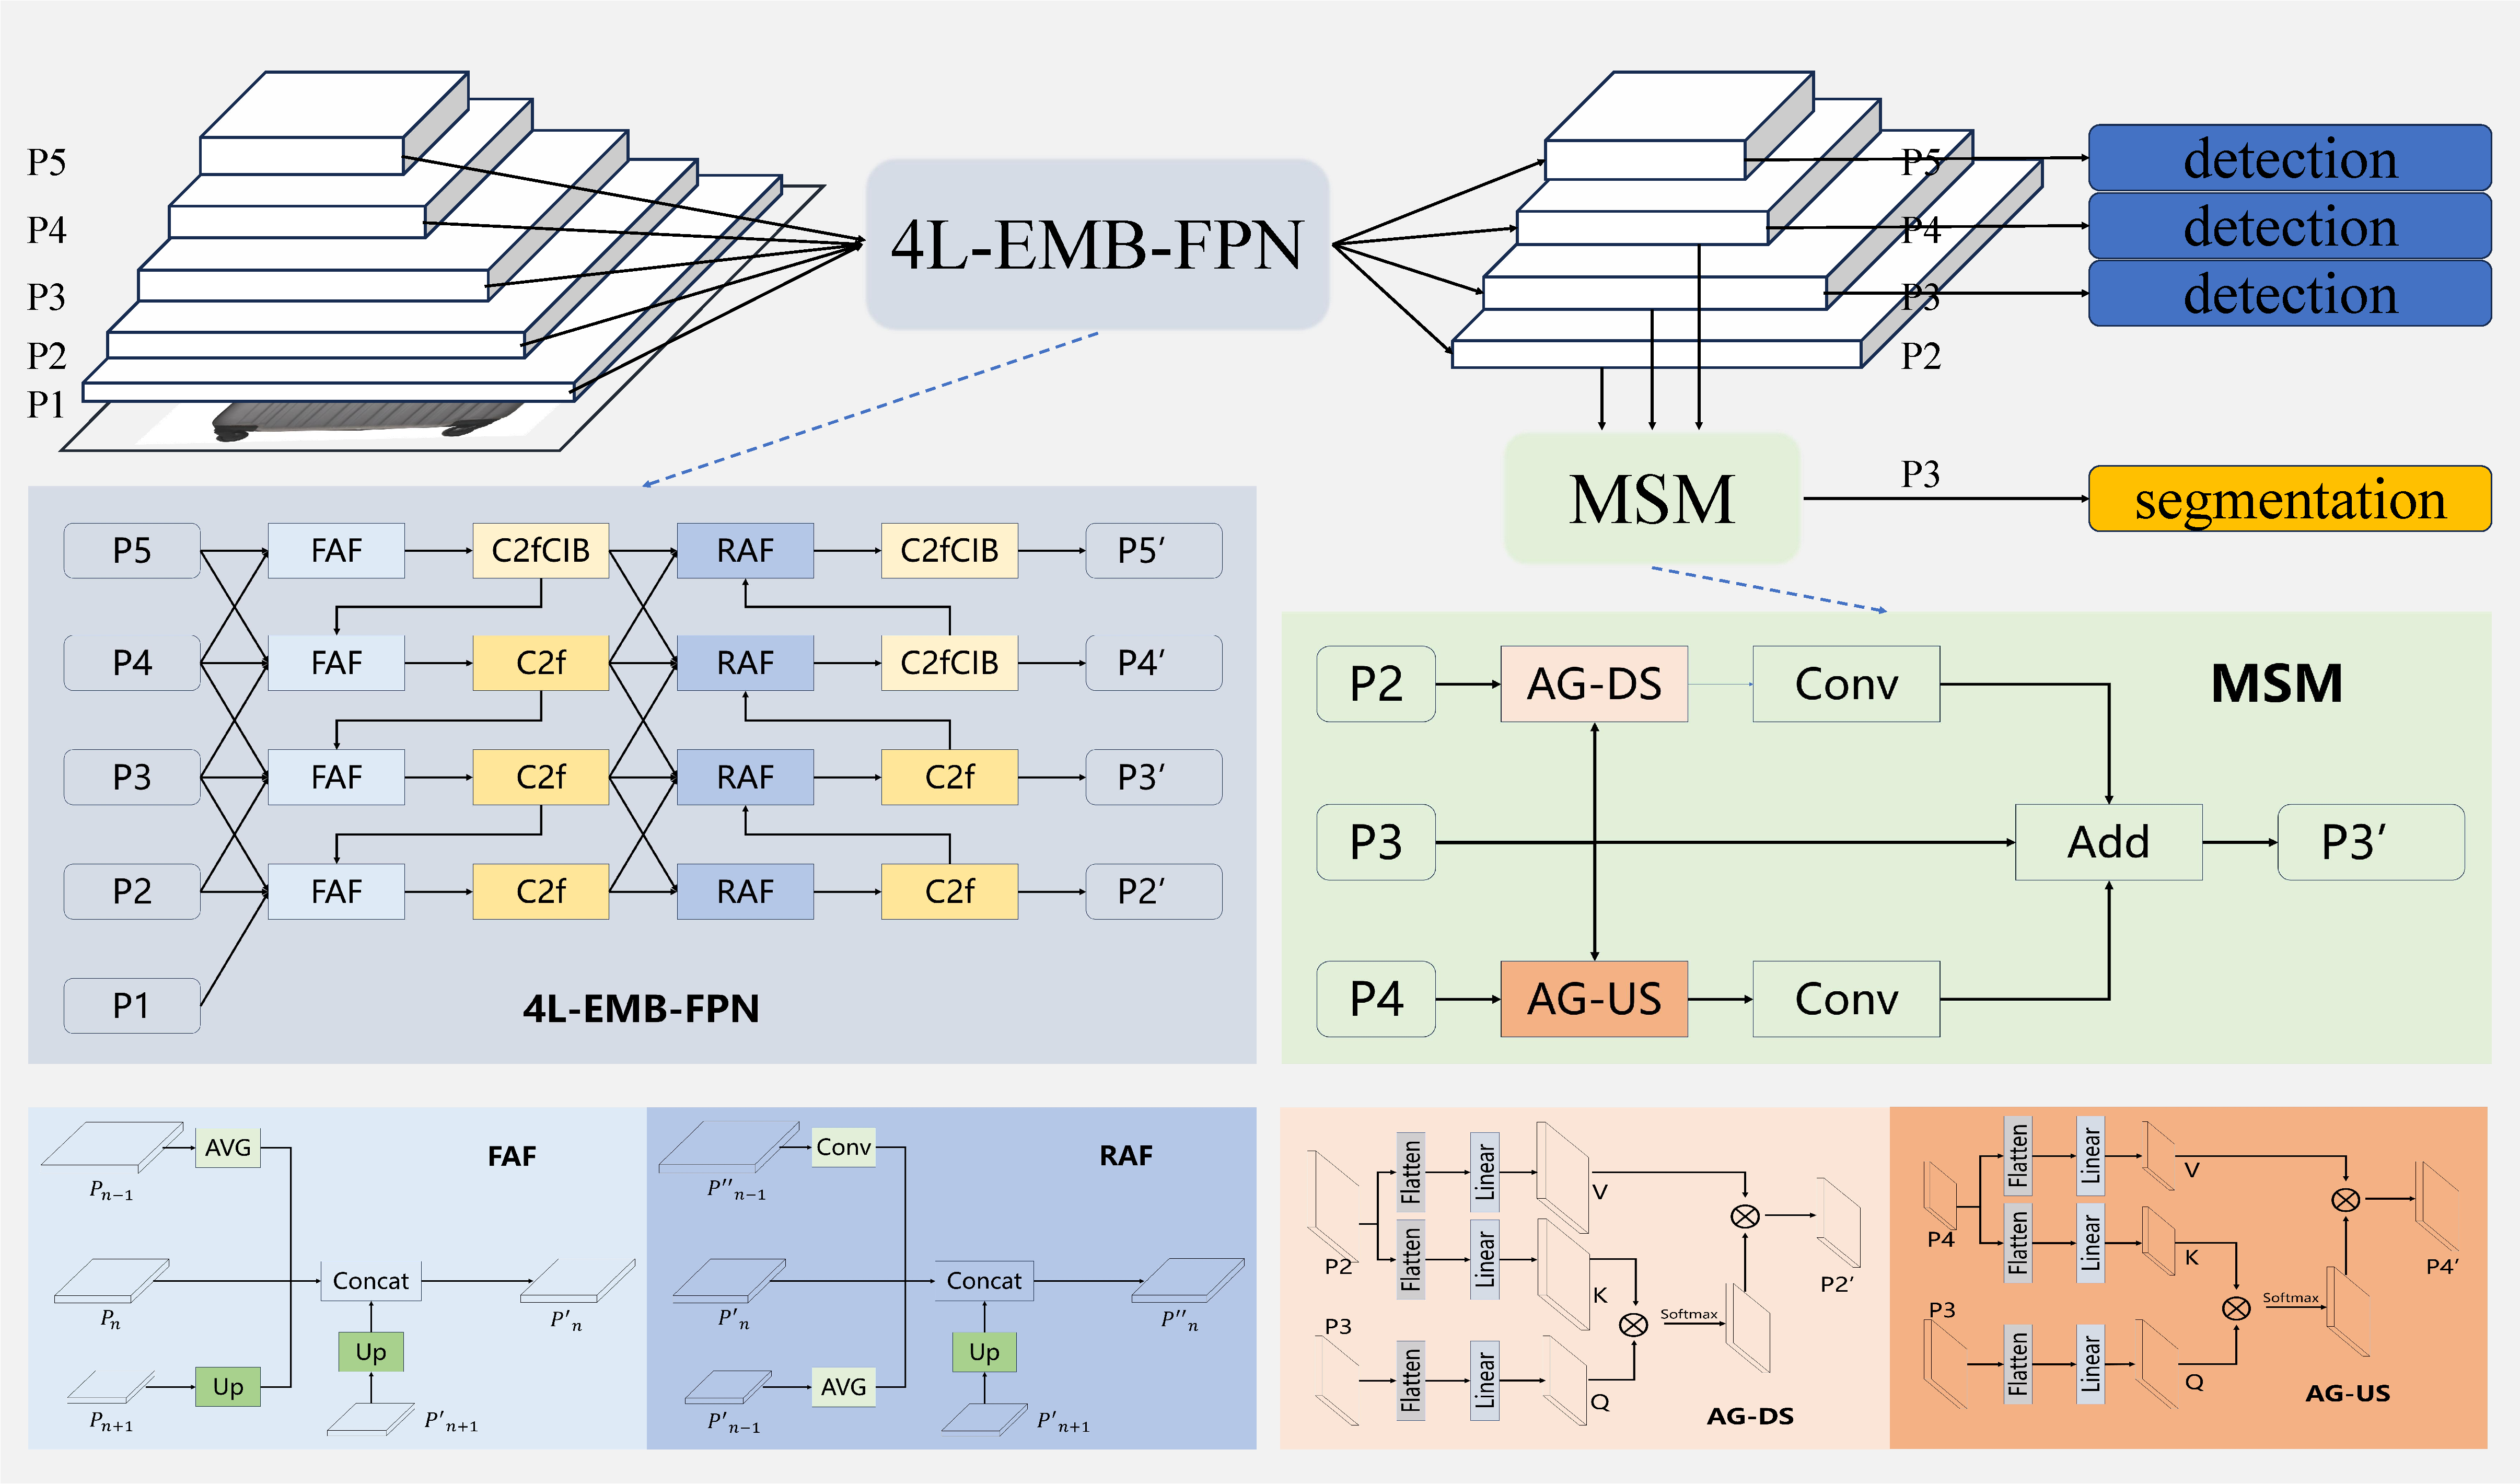
\includegraphics[width=\textwidth]{figures/fig2.pdf}
\caption{Schematic overview of the proposed MSAM-Net architecture.}
\label{fig:msam}
\end{figure*}

The 4L-EMB-FPN extracts four pyramid features, $P_2$--$P_5$, from the backbone. Low-level features preserve boundary details, whereas high-level features provide semantic context for large objects. To reduce semantic discrepancy between adjacent pyramid levels, a front-end aggregation fusion (FAF) module first aligns and fuses multi-level features. Given pyramid features $P_{n-1}$, $P_n$, $P_{n+1}$, and $P'_{n+1}$, FAF pools lower-level features, upsamples higher-level features, and concatenates them with $P_n$ to form an enriched representation $P'_n$. A refined aggregation fusion (RAF) module then further transforms, pools, upsamples, and concatenates these features to obtain $P''_n$. This two-stage fusion improves both large-instance semantic consistency and fine-grained boundary sensitivity.

\subsubsection{Attention-Guided Multi-Scale Mask Module}
Although the feature pyramid improves semantic representation, accurate mask reconstruction still requires explicit cross-scale interaction. The MSM uses $P_2$, $P_3$, and $P_4$ for mask prediction. Instead of using only interpolation or pooling, attention-guided downsampling (AG-DS) and attention-guided upsampling (AG-US) are used to exchange information between neighboring scales. In AG-DS, $P_3$ is projected as the query, while $P_2$ provides the key and value. In AG-US, $P_3$ is also used as the query, while $P_4$ provides the key and value. The attention operation is
\begin{equation}
\mathrm{Attention}(\boldsymbol{Q}_{x},\boldsymbol{K}_{y},\boldsymbol{V}_{y})=
\mathrm{Softmax}\left(\frac{\boldsymbol{Q}_{x}\boldsymbol{K}_{y}^{T}}{\sqrt{d}}\right)\boldsymbol{V}_{y},
\label{eq:attention}
\end{equation}
where $x\in\{\alpha,\beta\}$ indicates the downsampling or upsampling branch, $y\in\{2,4\}$ denotes the source pyramid level, and $d$ is the feature dimension. The attention outputs are reshaped and merged with the $P_3$ feature map.

To improve boundary regularity, an edge-aware mean-square error constraint is introduced using the distance field of the ground-truth boundary:
\begin{equation}
L_{\mathrm{MSE}}(\mathcal{B}_{\text{gt}},\mathcal{B}_{\text{pre}})=
\frac{1}{|\mathcal{B}_{\text{gt}}|}\sum_{\boldsymbol{p}\in\mathcal{B}_{\text{gt}}}d(\boldsymbol{p},\mathcal{B}_{\text{pre}})^{2},
\label{eq:mse}
\end{equation}
where $\mathcal{B}_{\text{gt}}$ and $\mathcal{B}_{\text{pre}}$ denote the ground-truth and predicted boundary-point sets, respectively, and $d(\boldsymbol{p},\mathcal{B}_{\text{pre}})$ is the shortest distance from point $\boldsymbol{p}$ to the predicted boundary.

\subsubsection{Training Objective}
The total loss combines standard detection losses with the segmentation constraint:
\begin{equation}
L_{\text{total}}=\lambda_{\text{box}}L_{\text{IOU}}+\lambda_{\text{seg}}L_{\text{seg}}+\lambda_{\text{cls}}L_{\text{cls}}+\lambda_{\text{dfl}}L_{\text{dfl}}.
\label{eq:loss}
\end{equation}
Here, $L_{\text{IOU}}$ is the CIoU-based box regression loss, $L_{\text{seg}}$ is the cropped mask reconstruction loss with the edge-aware boundary term, $L_{\text{cls}}$ is the BCE classification loss on task-aligned soft labels, and $L_{\text{dfl}}$ is the distribution focal loss for bounding-box localization. The weights $\lambda_{\text{box}}$, $\lambda_{\text{seg}}$, $\lambda_{\text{cls}}$, and $\lambda_{\text{dfl}}$ balance the four terms.

\begin{algorithm}[t]
\caption{Pixel-to-3D Cross Consistency Conditional Filtering (PX3C)}
\label{alg:px3c}
\begin{algorithmic}[1]

\Require Initial point cloud $P$ (masked by 2D results), thresholds
$\tau_{\mathrm{\text{thin}}},\tau_{\mathrm{\text{prot}}},\tau_{\mathrm{norm}}$

\Ensure Refined OBB $\mathrm{OBB}_{final}$, clean point set $P'$

\State \textbf{// Preprocessing Phase}

\State $P_{\text{down}} \gets \mathrm{VoxelGrid}(P)$
\State $P_{\text{rigid}} \gets \mathrm{RANSAC}(P_{\text{down}})$
    \Comment{Isolate luggage body}

\State $\mathrm{OBB}_{\text{cand}} \gets \mathrm{PCA}(P_{\text{rigid}})$
    \Comment{Initial candidate estimation}

\State $L_{\text{min}} \gets \mathrm{ShortestAxis}(\mathrm{OBB}_{\text{cand}})$

\State $P' \gets \emptyset$

\State \textbf{// Conditional Geometric Filtering Loop}

\ForAll{$p_i \in P_{\text{rigid}}$}

    \State Compute local neighborhood $\mathcal{N}(i)$,
           centroid $\bar{p}$, and normal $n$

    \State \textbf{// Feature 1: Thin Slice}

    \State
    $f_{\text{thin}}=\frac{\max_{p\in\mathcal{N}(i)}\langle\boldsymbol{p}-\bar{\boldsymbol{p}},\boldsymbol{n}\rangle-
\min_{p\in\mathcal{N}(i)}\langle\boldsymbol{p}-\bar{\boldsymbol{p}},\boldsymbol{n}\rangle}{L_{\min}}$

    \State \textbf{// Feature 2: Protrusion}

    \State
    $d_{\text{out}}(i)
    \gets
    \mathrm{SignedDistance}
    \!\left(
    p_i,
    \mathrm{surface}(OBB_{\text{cand}})
    \right)$

    \State
    $f_{\text{prot}}
    \gets
    \max\!\left\{0,\,
    \frac{d_{\text{out}}(i)}{\epsilon_{\text{prot}}}
    \right\}$

    \State \textbf{// Feature 3: Normal Consistency}

    \State
    $f_{\text{norm}}
    \gets
    1-\left|n_i\cdot n_{\text{body}}\right|$

    \State \textbf{// Filtering Condition: Remove if it matches tag/ribbon features}

    \If{$\neg \left(
            f_{\text{thin}}<\tau_{\text{thin}}
            \wedge
            f_{\text{prot}}>\tau_{\text{prot}}
            \wedge
            f_{\text{norm}}>\tau_{\text{norm}}
         \right)$}

        \State $P' \gets P' \cup \{p_i\}$
            \Comment{Keep points that are NOT tags/ribbons}

    \EndIf

\EndFor

\State \textbf{// Refined Reconstruction}

\State $\mathrm{OBB}_{\text{final}} \gets \mathrm{PCA}(P')$

\State \Return $\mathrm{OBB}_{\text{final}},\,P'$

\end{algorithmic}
\end{algorithm}

\subsection{Interference-Free 3D Modeling}
\subsubsection{PX3C Filtering}
Even after applying the 2D mask from Section 4.1, the projected point cloud often contains "ghost" points from unmasked ribbons or tag edges. To resolve this inconsistency between 2D segmentation and 3D geometry, we formulate the filtering process as a Conditional Geometric Self-Consistency problem. We employ standard preprocessing routines from the PCL, utilizing VoxelGrid downsampling for data regularization and RANSAC-based plane segmentation to isolate the rigid baggage body, and apply Principal Component Analysis (PCA) to construct the initial OBB $\mathcal{O}_{\text{cand}}$. However, Flexible attachments can still distort standard PCA, causing the OBB to misalign (e.g., the main axis following a drifting ribbon). This creates a circular dependency: accurate filtering requires a reliable model, but the model itself depends on filtered data. We address this via a self-bootstrapped conditional refinement (Algorithm~\ref{alg:px3c}), alternating between provisional model estimation and geometry-aware filtering.

\begin{algorithm}[t]
\caption{Consistency-Aware OBB Stabilization (CAOS)}
\label{alg:caos}
\begin{algorithmic}[1]

\Require Filtered point cloud $P_{\text{filt}}$,
current raw observation $b_t^{\text{raw}}$,
previous state $b_{t-1}$,
last stable snapshot $b^{*}$,
conveyor velocity $v$,
quality threshold $q_{\text{min}}$

\Ensure Stabilized OBB state $b_t$

\State \textbf{// Quality Assessment Phase}

\State
$C_{\text{main}}
\gets
\mathrm{EuclideanCluster}(P_{\text{filt}})$
\Comment{Largest connected component}

\State
$q_{\text{cov}}
\gets
\frac{|C_{\text{main}}|}{|P_{\text{filt}}|}$

\State
$q_{\text{in}}
\gets
\frac{
\left|
\left\{
p\in C_{\text{main}} :
d(p,O_t)\le \tau_{\text{in}}
\right\}
\right|
}
{|C_{\text{main}}|}
$

\State
\[
q_{\text{stab}}
\gets
\exp\!\left(
-\frac{
w_p\|\Delta P\|^2
+
w_r\|\Delta R\|^2
+
w_s\|\Delta S\|^2
}
{\eta}
\right)
\]

\State
$q
\gets
\alpha_1 q_{\text{cov}}
+
\alpha_2 q_{\text{in}}
+
\alpha_3 q_{\text{stab}}$

\State \textbf{// Adaptive Smoothing Weight}

\State
$\beta(q)
\gets
\min\!\left(
\beta_{\text{max}},
k(1-q)
\right)$

\State \textbf{// Dynamic State Update Strategy}

\If{$q<q_{\text{min}}$}

    \State \textbf{// Low Quality: Extrapolate from Last Stable State}

    \State
    $\Delta t_{\text{gap}}
    \gets
    \mathrm{TimeSince}(b^{*})$

    \State
    $b_t
    \gets
    b^{*}
    \oplus
    \left(v\cdot\Delta t_{\text{gap}}\right)$

\Else

    \State \textbf{// High Quality: Adaptive Smoothing}

    \State
    \[
    b_t
    \gets
    \left(1-\beta(q)\right)b_t^{\text{raw}}
    +
    \beta(q)
    \left(
    b_{t-1}
    \oplus
    (v\cdot\Delta t)
    \right)
    \]

    \State
    $b^{*} \gets b_t$
    \Comment{Update reference snapshot}

\EndIf

\State \Return $b_t$

\end{algorithmic}
\end{algorithm}

\begin{figure}[!t]
\centering
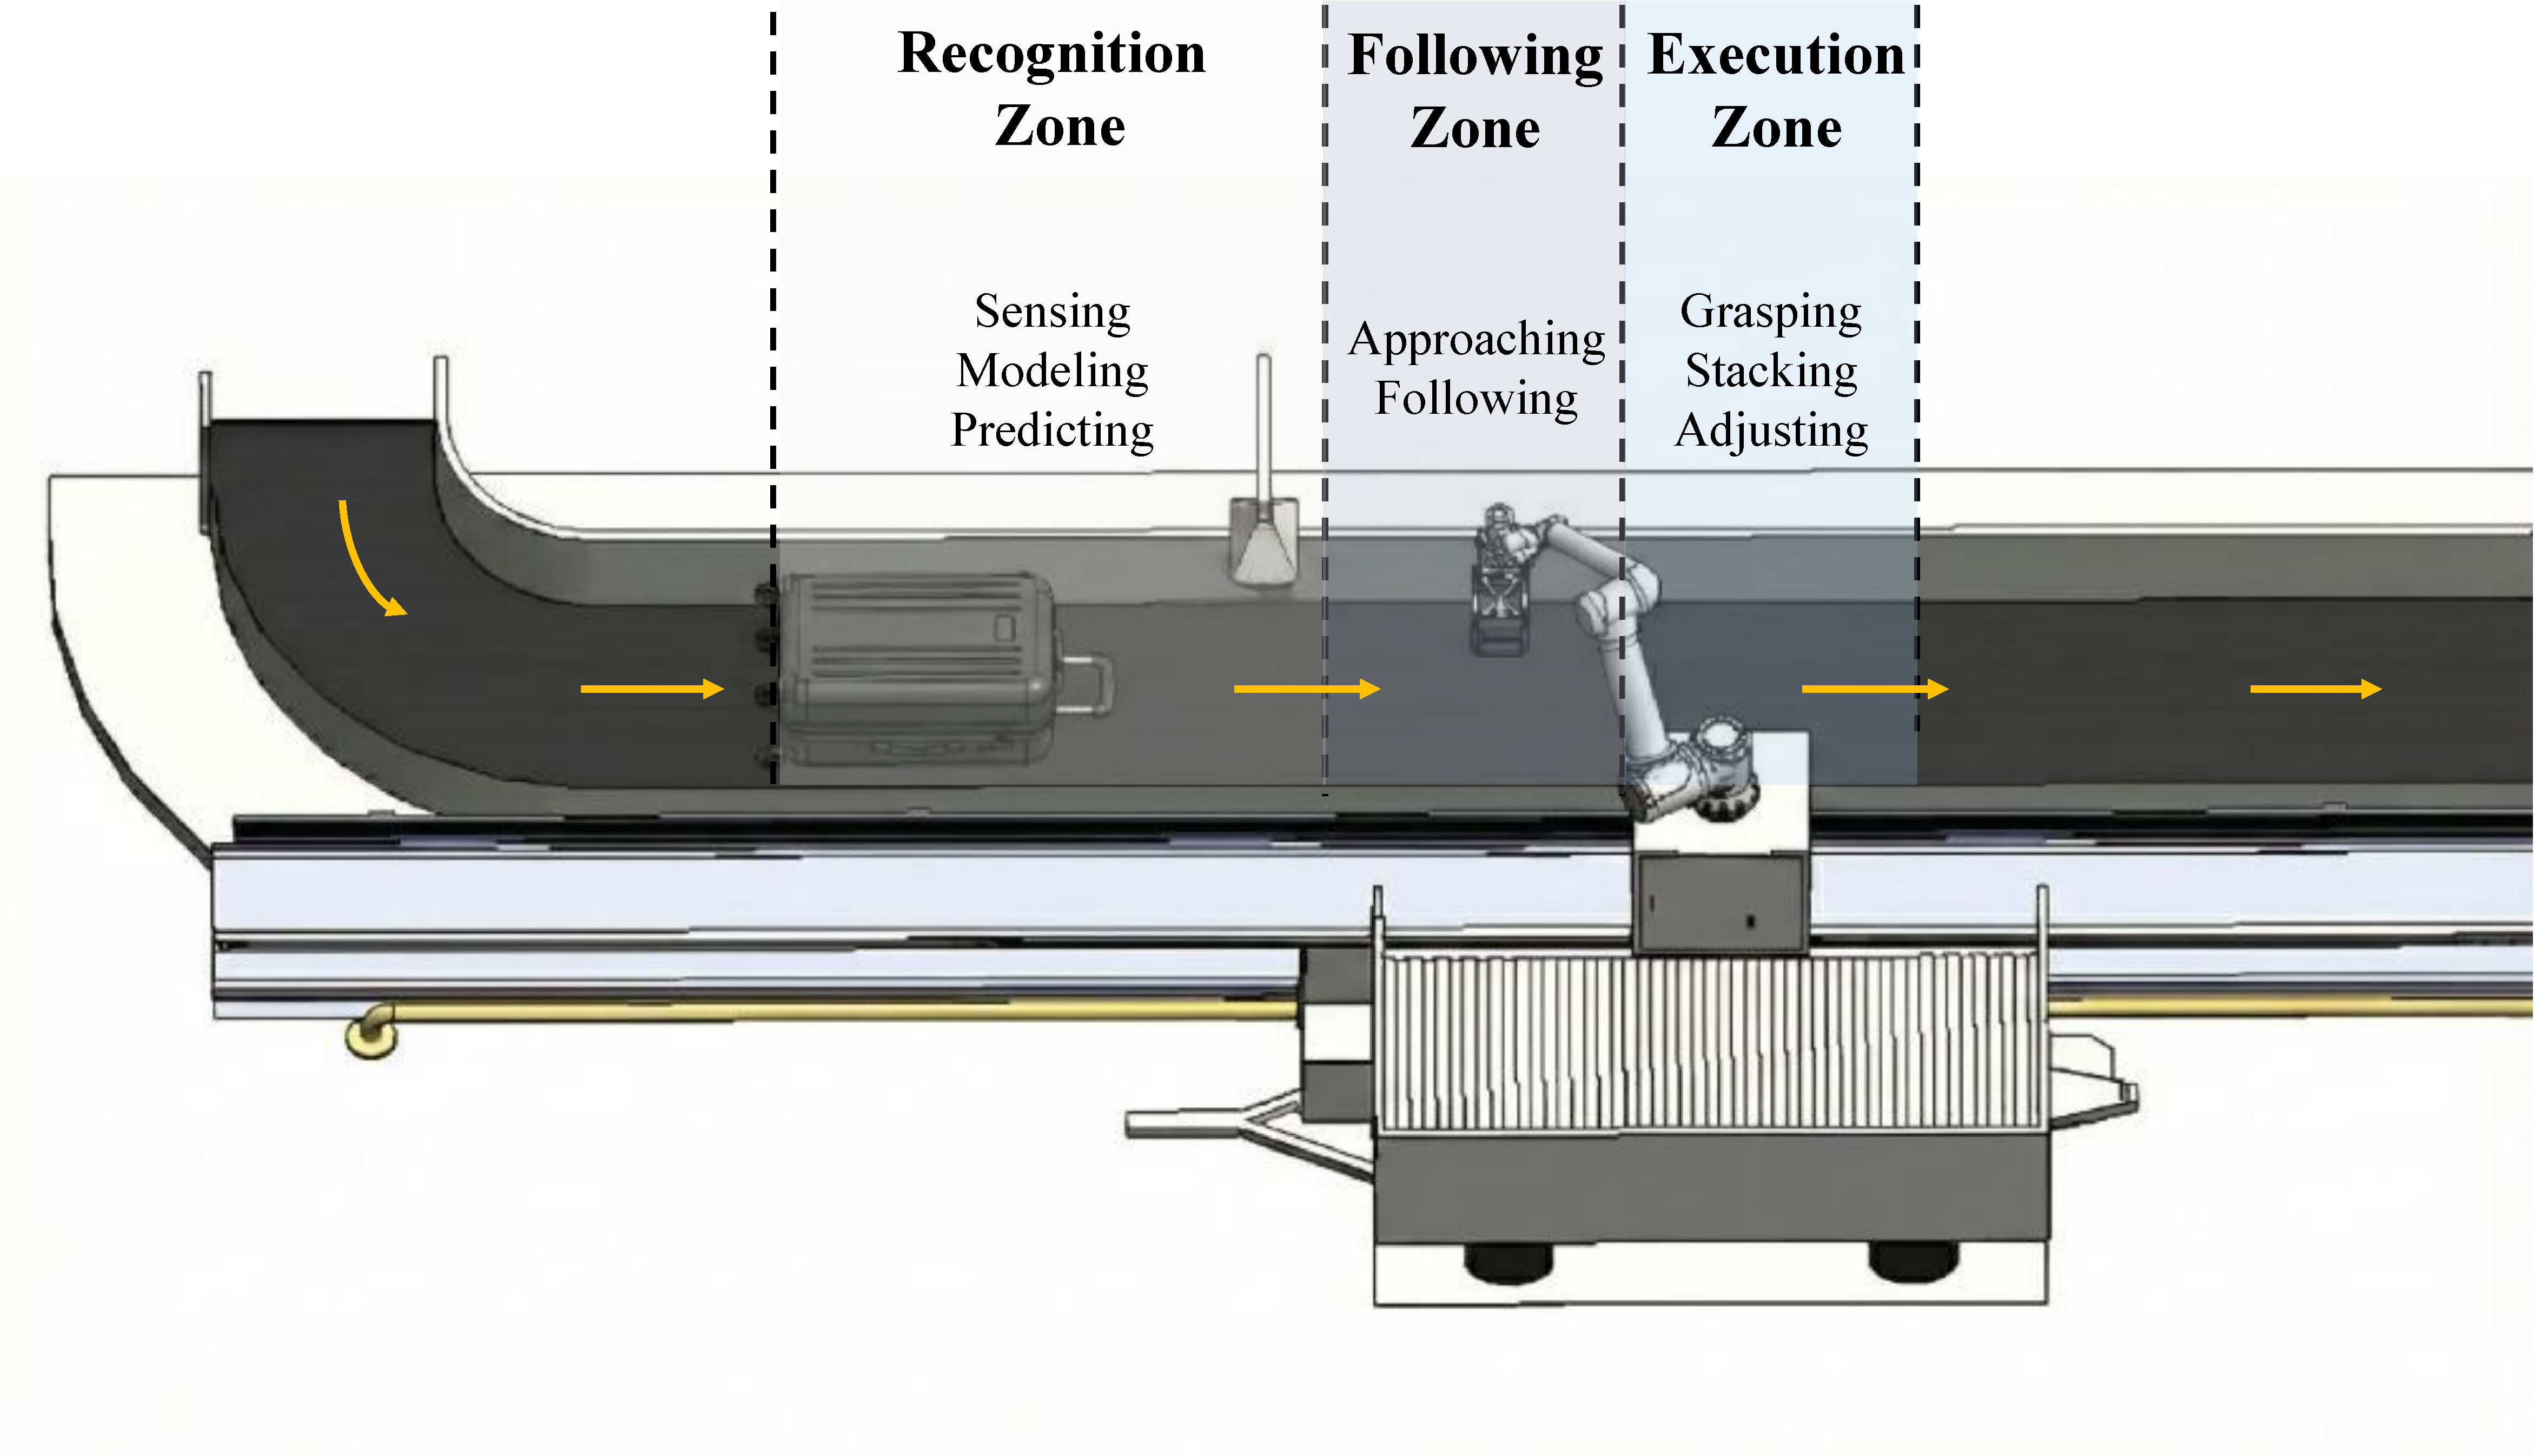
\includegraphics[width=\columnwidth]{figures/fig3.pdf}
\caption{System Workflow of the Dynamic Grasping Strateg.}
\label{fig:planning}
\end{figure}

For each point $P_i$, three features are computed. The thin-slice feature evaluates the local thickness relative to the shortest OBB dimension $L_{\min}$:
\begin{equation}
f_{\text{thin}}=\frac{\max_{p\in\mathcal{N}(i)}\langle\boldsymbol{p}-\bar{\boldsymbol{p}},\boldsymbol{n}\rangle-
\min_{p\in\mathcal{N}(i)}\langle\boldsymbol{p}-\bar{\boldsymbol{p}},\boldsymbol{n}\rangle}{L_{\min}},
\label{eq:fthin}
\end{equation}
where $\mathcal{N}(i)$ is the local neighborhood, $\bar{\boldsymbol{p}}$ is the neighborhood centroid, and $\boldsymbol{n}$ is the average normal. The protrusion feature measures the normalized distance outside the provisional OBB:
\begin{equation}
f_{\text{\text{prot}}}=\max\{0,d_{\text{\text{out}}}(i)/\epsilon_{\text{\text{prot}}}\},
\label{eq:fprot}
\end{equation}
where $d_{\text{out}}(i)$ is the signed distance to the OBB surface. The normal-consistency feature is
\begin{equation}
f_{\text{norm}}=1-|\boldsymbol{n}_{i}\cdot\bar{\boldsymbol{n}}|,
\label{eq:fnorm}
\end{equation}
where $\boldsymbol{n}_{i}$ is the local normal and $\bar{\boldsymbol{n}}$ is the dominant surface normal. Points satisfying the combined flexible-interference condition are removed, and PCA is applied again to reconstruct the refined OBB. This self-bootstrapped refinement reduces the effect of residual 2D segmentation leakage and produces a rigid-body representation more suitable for grasp planning.

\subsubsection{CAOS Temporal Stabilization}
Single-frame OBB estimates may still fluctuate because of motion blur, occlusion, or depth noise. To prevent erratic control commands, we employ the CAOS method (see Algorithm~\ref{alg:caos}), which utilizes multi-frame consistency for stabilization. CAOS stabilizes the OBB sequence using quality-aware temporal smoothing. Let $\mathcal{P}_{\text{filt}}$ be the filtered point cloud and $\mathcal{C}_{\text{main}}\subseteq\mathcal{P}_{\text{filt}}$ be the largest connected component. The coverage score and inlier-rate score are defined as
\begin{equation}
q_{\text{cov}}=\frac{|\mathcal{C}_{\text{\text{main}}}|}{|\mathcal{P}_{\text{\text{filt}}}|},\quad
q_{\text{in}}=\frac{\left|\{p\in\mathcal{C}_{\text{\text{main}}}:d(p,\mathcal{O}_{t})\le\tau_{\text{\text{in}}}\}\right|}{|\mathcal{C}_{\text{\text{main}}}|}.
\label{eq:qcov}
\end{equation}
The first score measures whether the point cloud is dominated by one coherent object, while the second measures how well the estimated OBB fits the observed points. Temporal stability is quantified as
\begin{equation}
q_{\text{\text{stab}}}=\exp\left(-\frac{w_p\|\Delta\boldsymbol{P}\|^2+w_r\|\Delta\boldsymbol{R}\|^2+w_s\|\Delta\boldsymbol{S}\|^2}{\eta}\right),
\label{eq:qstab}
\end{equation}
where $\Delta\boldsymbol{P}$, $\Delta\boldsymbol{R}$, and $\Delta\boldsymbol{S}$ denote changes in position, rotation, and scale. The aggregate quality score is written as:
\begin{equation}
q=\alpha_1q_{\text{cov}}+\alpha_2q_{\text{\text{in}}}+\alpha_3q_{\text{\text{stab}}}.
\end{equation}
and the output OBB state is updated by:
\begin{equation}
\boldsymbol{b}_{t}=\begin{cases}
\boldsymbol{b}^{*}\oplus(\boldsymbol{v}\Delta t_{\text{gap}}), & q<q_{\text{\text{min}}},\\
(1-\beta(q))\boldsymbol{b}_{t}^{\text{raw}}+\beta(q)(\boldsymbol{b}_{t-1}\oplus(\boldsymbol{v}\Delta t)), & \mathrm{otherwise},
\end{cases}
\label{eq:caos}
\end{equation}
where $\boldsymbol{b}^{*}$ is the last reliable snapshot, $\boldsymbol{b}_{t}^{\text{raw}}$ is the current PX3C observation, $\oplus(\boldsymbol{v}\Delta t)$ denotes conveyor-motion compensation over duration $\Delta t$, and $\beta(q)=\min(\beta_{\text{\text{max}}},k(1-q))$ is an adaptive smoothing coefficient. A lower quality score increases the reliance on historical prediction, thereby preventing abrupt and unreliable control commands.

\begin{figure}[!t]
\centering
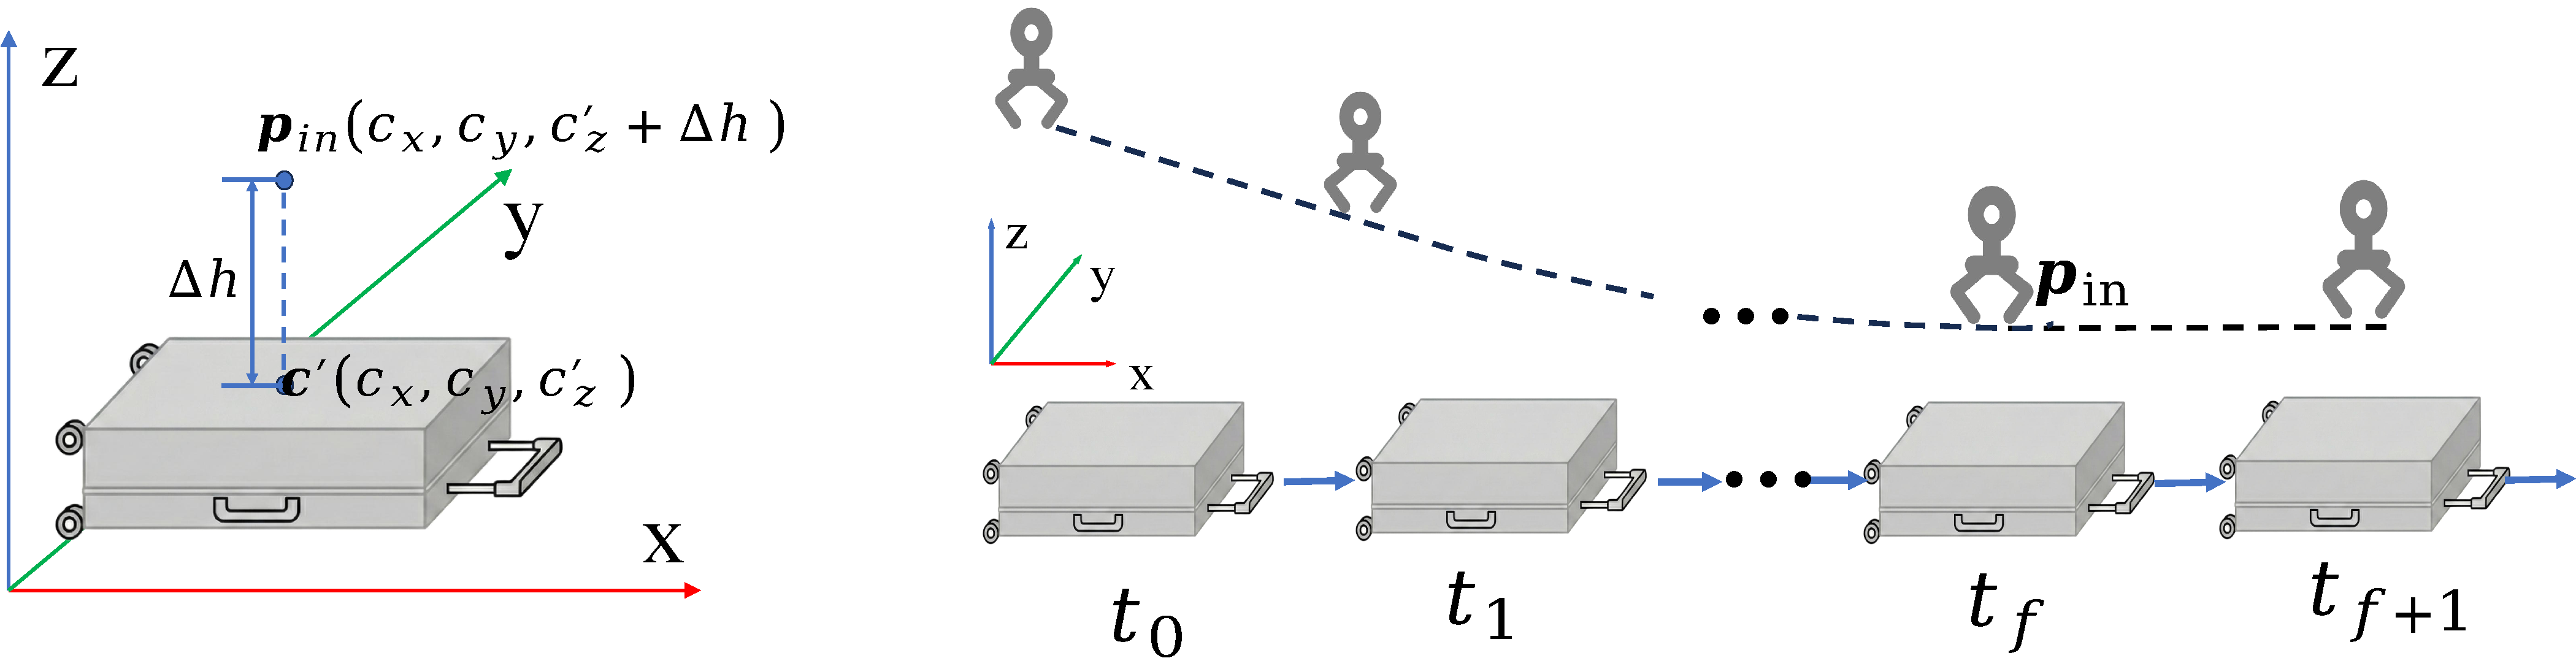
\includegraphics[width=\columnwidth]{figures/fig4.pdf}
\caption{Schematic Diagram of the Interception Point $P_{\text{\text{in}}}$ and Rapid Interception Strategy.}
\label{fig:rapid_interception}
\end{figure}

\subsection{Dynamic Grasping and Active Interaction}
We adopt a "Predict-Follow-Grasp" execution paradigm, as illustrated in Fig. \ref{fig:planning}. The process involves visual perception and modeling in the Recognition Zone, followed by velocity synchronization in the Following Zone, and finally, grasping execution in the Execution Zone.
\subsubsection{Recursive Bayesian State Estimation}
The dynamic state of the baggage centroid is estimated using a discrete Kalman filter with a constant-acceleration model. The state vector is
\begin{equation}
\boldsymbol{x}_{k}=[p_x,v_x,a_x,p_y,v_y,a_y,p_z,v_z,a_z]^T.
\end{equation}
The process and observation models are
\begin{equation}
\begin{cases}
\boldsymbol{x}_{k}=\boldsymbol{F}\boldsymbol{x}_{k-1}+\boldsymbol{w}_{k-1},\\
\boldsymbol{z}_{k}=\boldsymbol{H}\boldsymbol{x}_{k}+\boldsymbol{v}_{k},
\end{cases}
\label{eq:state}
\end{equation}
where $\boldsymbol{z}_{k}$ is the observed centroid, $\boldsymbol{w}_{k-1}\sim\mathcal{N}(0,\boldsymbol{Q})$ is the process noise, and $\boldsymbol{v}_{k}\sim\mathcal{N}(0,\boldsymbol{R})$ is the measurement noise. The transition matrix is block diagonal:
\begin{equation}
\boldsymbol{F}=\mathrm{diag}(\boldsymbol{F}_{x},\boldsymbol{F}_{y},\boldsymbol{F}_{z}),
\end{equation}
with
\begin{equation}
\boldsymbol{F}_{x}=\begin{bmatrix}
1 & \Delta T & \frac{1}{2}\Delta T^{2}\\
0 & 1 & \Delta T\\
0 & 0 & 1
\end{bmatrix}.
\label{eq:fx}
\end{equation}
The filter operates in a \textit{Predict-Update} cycle. In the \textit{Predict} phase, we extrapolate the prior state $\hat{\boldsymbol{x}}_{k}^{-}$ and the error covariance $\boldsymbol{P}_{k}^{-}$ based on the optimal estimation from the previous step:
\begin{equation}
\hat{\boldsymbol{x}}_{k}^{-}=\boldsymbol{F}\hat{\boldsymbol{x}}_{k-1},\
\boldsymbol{P}_{k}^{-}=\boldsymbol{F}\boldsymbol{P}_{k-1}\boldsymbol{F}^{T}+\boldsymbol{Q},
\end{equation}
and in the \textit{Update} phase, the Kalman Gain $\boldsymbol{K}_{k}$ is computed using the current observation $\boldsymbol{z}_k$ to correct the prior error, yielding the optimal posterior estimation $\boldsymbol{x}_k$ and the updated posterior error covariance $\boldsymbol{P}_{k}$ as:
\begin{equation}
\begin{cases}
    \boldsymbol{K}_{k}=\boldsymbol{P}_{k}^{-}\boldsymbol{H}^{T}(\boldsymbol{H}\boldsymbol{P}_{k}^{-}\boldsymbol{H}^{T}+\boldsymbol{R})^{-1}, \\
\hat{\boldsymbol{x}}_{k}=\hat{\boldsymbol{x}}_{k}^{-}+\boldsymbol{K}_{k}(\boldsymbol{z}_{k}-\boldsymbol{H}\hat{\boldsymbol{x}}_{k}^{-}), \\
\boldsymbol{P}_{k}=(\boldsymbol{I}-\boldsymbol{K}_{k}\boldsymbol{H})\boldsymbol{P}_{k}^{-}.
\end{cases}
\end{equation}
The trace of $\boldsymbol{P}_{k}$ is used as an uncertainty indicator. When collision, sliding, or occlusion causes the observation model to fail, the uncertainty increases and can trigger active state regulation. This serves as a robust metric to determine whether the target is maintaining stable motion. 

For rotation prediction, since rotation on conveyor belts is typically gradual, we apply the same smoothing filter as the position estimation to the components of the quaternion $\boldsymbol{q}_t$. Finally, the target position for a future timestamp $t_p$ is computed as:
\begin{equation}
\boldsymbol{c}(t_p)=\hat{\boldsymbol{p}}_{\text{now}}+\hat{\boldsymbol{v}}_{\text{now}}(t_p-t_{\text{now}})+\frac{1}{2}\hat{\boldsymbol{a}}_{\text{now}}(t_p-t_{\text{now}})^2.
\end{equation}
Quaternion components $\boldsymbol{q}(t_p)$ are normalized before conversion to the rotation matrix with $\boldsymbol{R}(t_p) = \mathrm{quat2rot}(\frac{\boldsymbol{q}(t_p)}{\left \| \boldsymbol{q}(t_p) \right \| })$ for the robot controller.

\subsubsection{Coarse-to-Fine Planning in Relative Velocity Space}
The grasping planner contains two stages, as shown in Algorithm~\ref{algo:two_stage_dynamic_grasping}. Stage I performs rapid interception. The end-effector moves from $\boldsymbol{p}_{\text{start}}$ to an ``interception point" $\boldsymbol{p}_{\text{in}}$ above the predicted target trajectory in minimal time (as shown in Fig.~\ref{fig:rapid_interception}). Rather than solving a full dynamic trajectory optimization problem, the earliest interception time $t_f$ is estimated from
\begin{equation}
\|\boldsymbol{p}(t_f)-\boldsymbol{p}_{\text{start}}\|-\bar{\boldsymbol{v}}(t_f-t_{\text{start}})=0,
\label{eq:interception}
\end{equation}
where $\bar{\boldsymbol{v}}$ is the average feasible robot velocity. \eqref{eq:interception} is solved iteratively using Newton--Raphson updates. To compensate for neglected acceleration and jerk constraints, a buffer term is added:
\begin{equation}
t_f'=t_f+\Delta t_{\text{buffer}},\quad
\Delta t_{\text{buffer}}=\alpha\frac{v_{\text{\text{max}}}}{a_{\text{\text{max}}}}, \label{equ:estimate}
\end{equation}
where $\alpha$ is a safety factor set to 1.2.

\begin{figure}[!t]
\centering
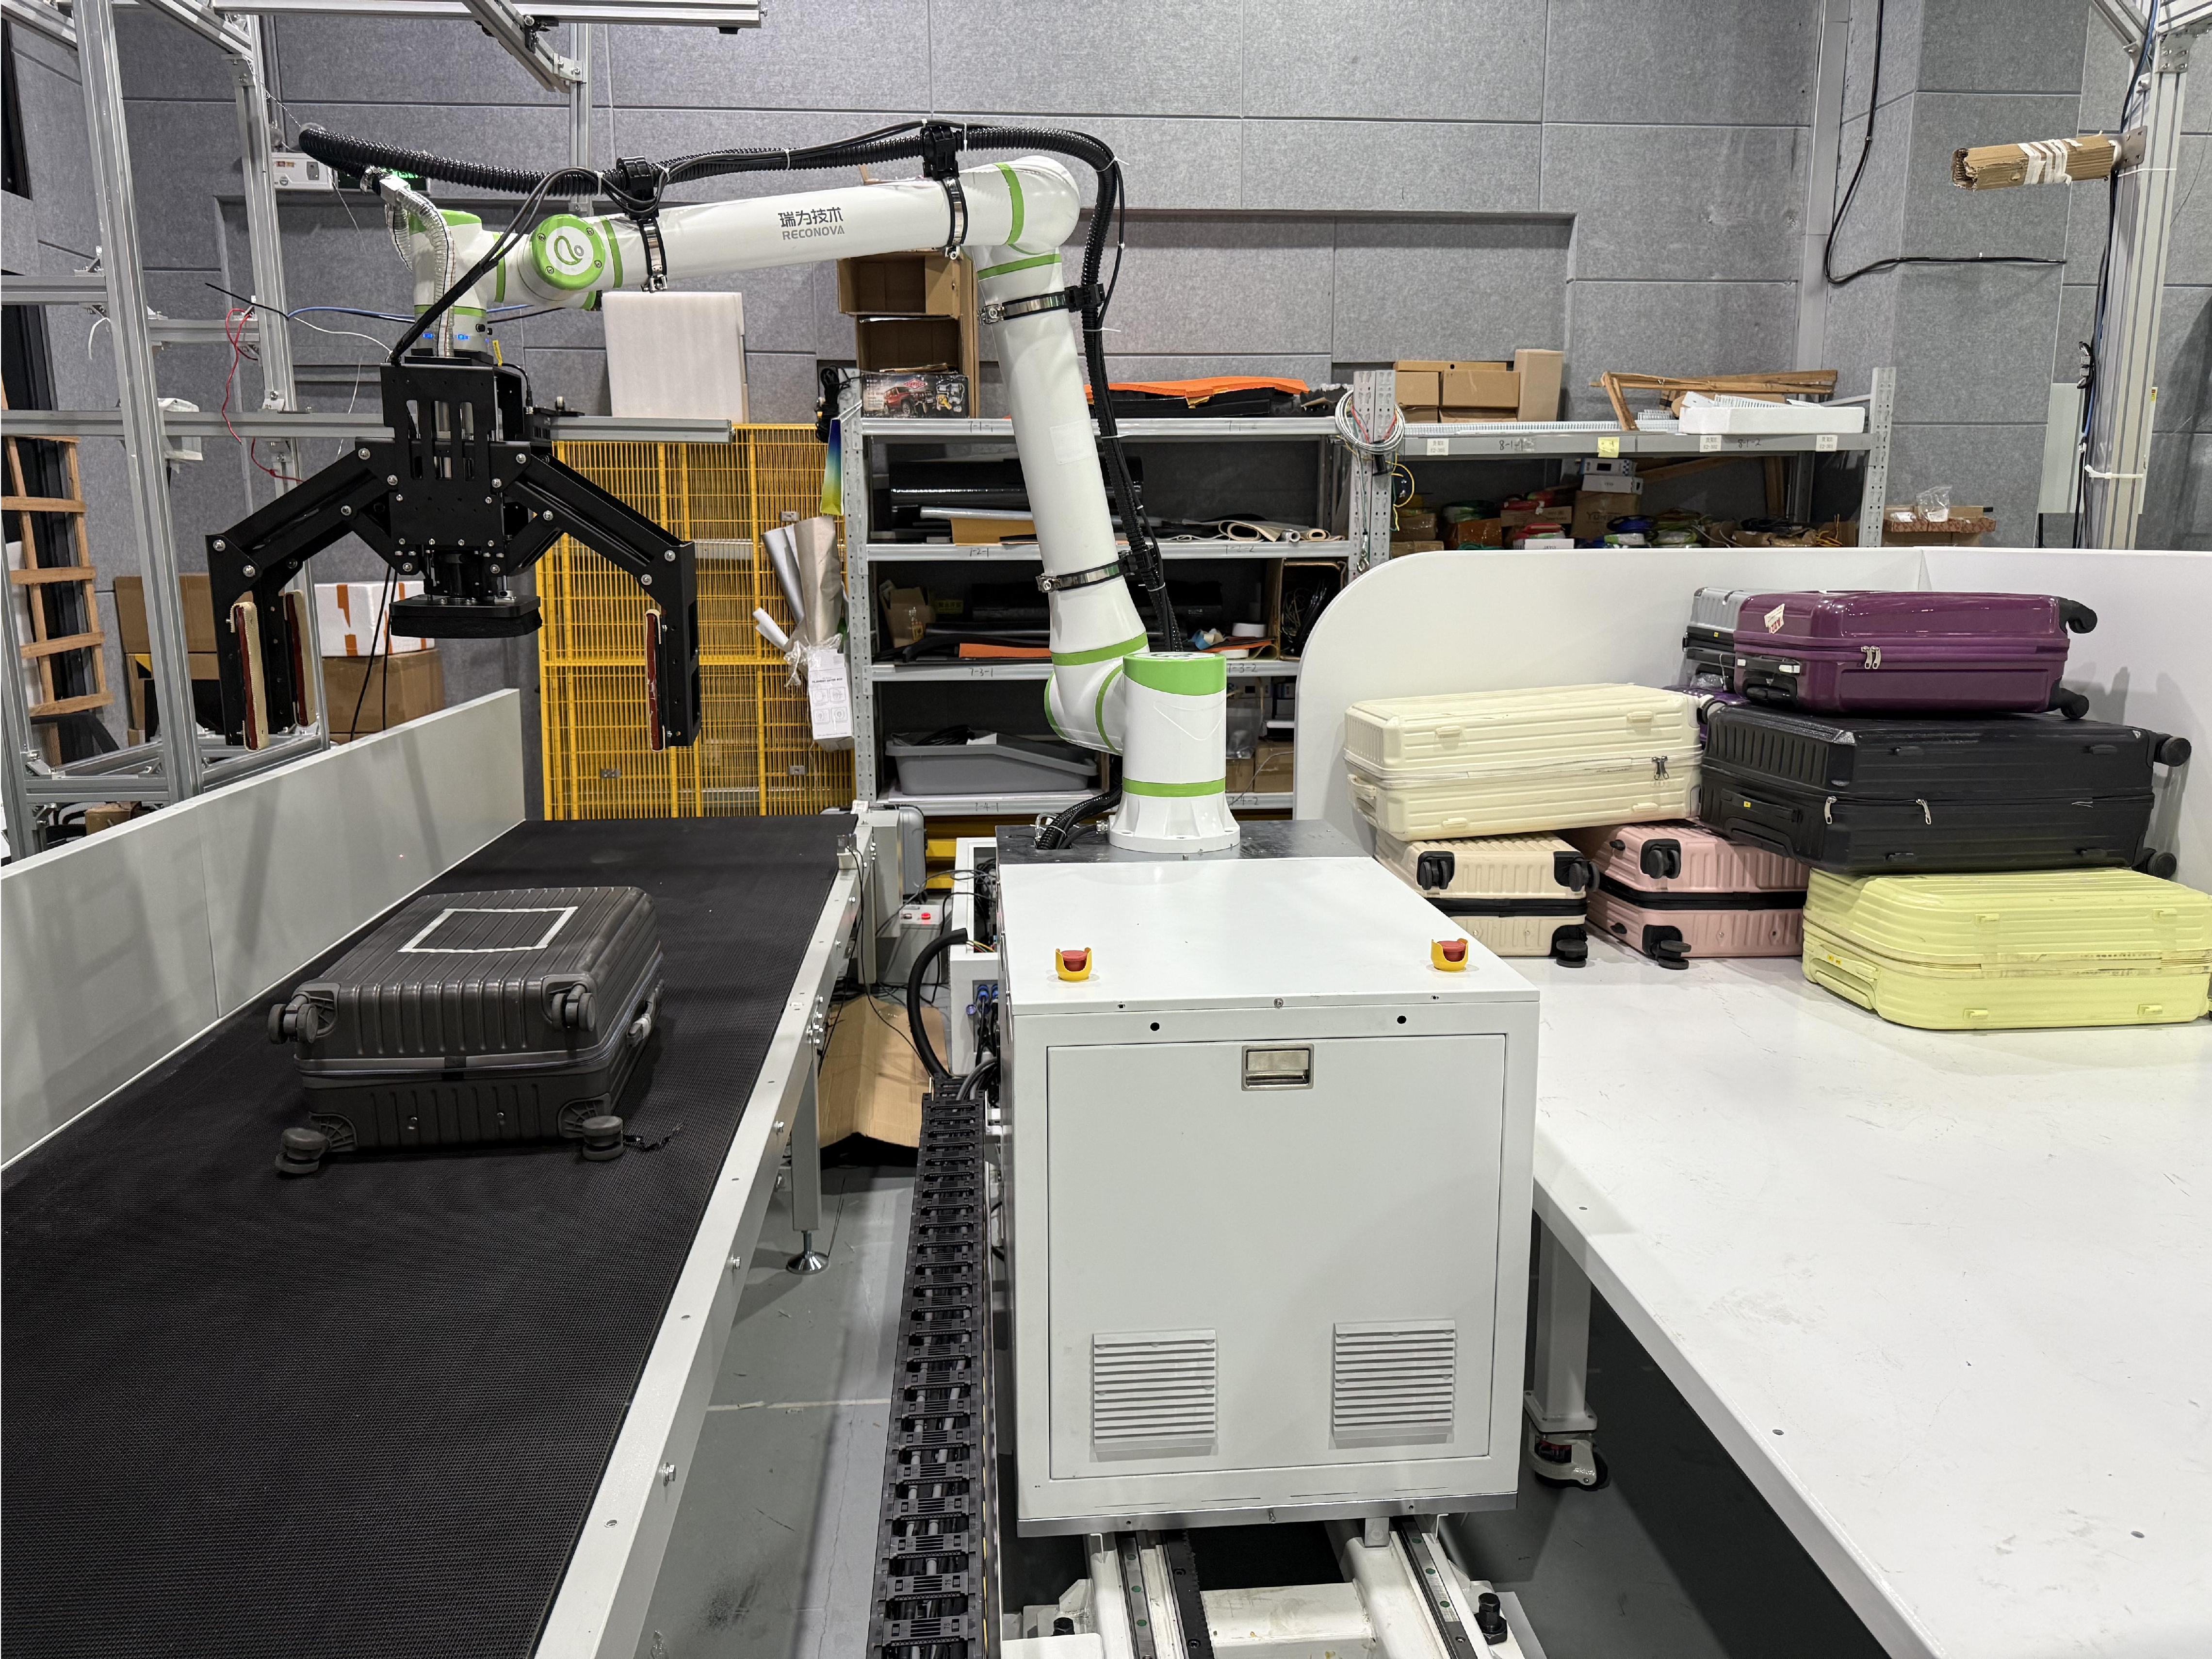
\includegraphics[width=\columnwidth]{figures/fig5.pdf}
\caption{Robotic baggage-handling platform.}
\label{fig:setup}
\end{figure}

Stage II performs fine synchronization in relative velocity space. The dynamic grasping task is converted into a relative alignment problem by minimizing
\begin{equation}
E_{\text{sync}}(t)=\frac{\|\boldsymbol{v}_{\text{EE}}(t)-\boldsymbol{v}_{\text{grasp}}(t)\|^2}{v_{\text{ref}}^{2}}+
\lambda\frac{\|\boldsymbol{p}_{\text{EE}}^{xy}(t)-\boldsymbol{p}_{\text{grasp}}^{xy}(t)\|^2}{d_{\text{ref}}^{2}}.
\label{eq:sync}
\end{equation}
The first term measures velocity synchronization, and the second term measures planar position alignment. When $E_{\text{sync}}<\epsilon_{\text{safe}}$, the end-effector and target are treated as relatively static, and the robot performs the final short vertical descent. Because the descent distance is only 80$\mathrm{mm}$, the residual relative velocity is negligible during this interval. The final motion is therefore planned as a local point-to-point trajectory using a quintic polynomial.

\begin{algorithm}[t]
\caption{Two-Stage Dynamic Grasping Planning Strategy}
\label{algo:two_stage_dynamic_grasping}
\begin{algorithmic}[1]

\Require Target state estimate
$\hat{\mathbf{x}}_k=
[\mathbf{p}_{\text{obj}},\mathbf{v}_{\text{obj}}]^{T}$;
robot kinematic limits $v_{\text{max}},a_{\text{max}}$;
thresholds $\epsilon_{\text{safe}},\lambda,v_{\text{ref}},d_{\text{ref}}$

\Ensure Robot position command vector $\mathbf{q}_{\text{cmd}}$

\State \textbf{// Stage 1: Fast Interception (Coarse Planning)}

\State Define interception offset point
$P_{\text{in}}=\mathbf{p}_{\text{obj}}+[0,0,\Delta h]^{T}$

\State Initialize $t_f$ using heuristic estimation

\Repeat

    \State Update $t_f$ using Newton--Raphson on distance constraint:

    \State
    $f(t)=
    \left\|
    \mathbf{p}_{\text{obj}}(t)-P_{\text{start}}
    \right\|
    -
    v_{\text{avg}}\cdot t$

\Until{convergence}

\State Apply buffer term:
$t_{\text{inter}}\gets t_f+\alpha\frac{v_{\text{max}}}{a_{\text{max}}}$

\State Execute trajectory to reach $P_{\text{in}}$ at time $t_{\text{inter}}$

\State \textbf{// Stage 2: Synchronization (Relative Velocity Space)}

\While{grasp not completed}

    \State Obtain real-time error vectors
    $\mathbf{v}_{\text{err}},\mathbf{p}_{\text{err}}$

    \State Compute normalized synchronization cost $E_{\text{sync}}$:

    \State
    $E_{\text{sync}}
    \gets
    \frac{\left\|\mathbf{v}_{\text{err}}\right\|^2}{v_{\text{ref}}^{2}}
    +
    \lambda
    \frac{\left\|\mathbf{p}_{\text{err}}\right\|^2}{d_{\text{ref}}^{2}}$

    \If{$E_{\text{sync}}<\epsilon_{\text{safe}}$}
        \Comment{Condition met: relative static state}

        \State Trigger Z-axis descent to target surface

        \State Close gripper

        \State \Return success

    \Else

        \State Compute control input to minimize $E_{\text{sync}}$

        \State Update $\mathbf{q}_{\text{cmd}}$ via inverse kinematics

    \EndIf

\EndWhile

\end{algorithmic}
\end{algorithm}

\subsubsection{Active State Regulation}
Passive visual servoing assumes that observation uncertainty will eventually decrease as additional frames are received. This assumption is not always valid in conveyor-belt baggage handling. Stacked or colliding objects may remain in high-entropy states, causing the posterior covariance of the Kalman filter to diverge or the synchronization objective to fail. The proposed active interaction mechanism addresses this failure mode by allowing the robot to reshape the environment. When $\mathrm{tr}(\boldsymbol{P}_{k})$ exceeds a safety threshold or $E_{\text{sync}}$ does not converge, precision placement is temporarily aborted. The robot then performs a best-effort suction grasp based on the predicted centroid and relocates the baggage to an empty conveyor region detected by the vision system. This reset action converts a chaotic or poorly observable state into an ordered state for subsequent handling, thereby closing the loop between perception and manipulation.
\section{Experiments and Results}
\subsection{Experimental Setup}
The proposed framework was deployed on a real robotic baggage-handling platform, shown in Fig.~\ref{fig:setup}. The platform consists of a collaborative robotic arm equipped with a hybrid suction--gripper end-effector, a conveyor belt operating at 493~mm/s, and an Orbbec Gemini 435Le RGB-D camera with a resolution of $640\times400$ at 20~FPS. All algorithms were executed on an embedded AX650N processor. MSAM-Net inference, PX3C filtering, and CAOS stabilization were executed at every frame. DKF state prediction was executed every five frames, corresponding to approximately 200$\mathrm{ms}$ and a conveyor displacement of about 98.6~mm.

\begin{figure}[!t]
\centering
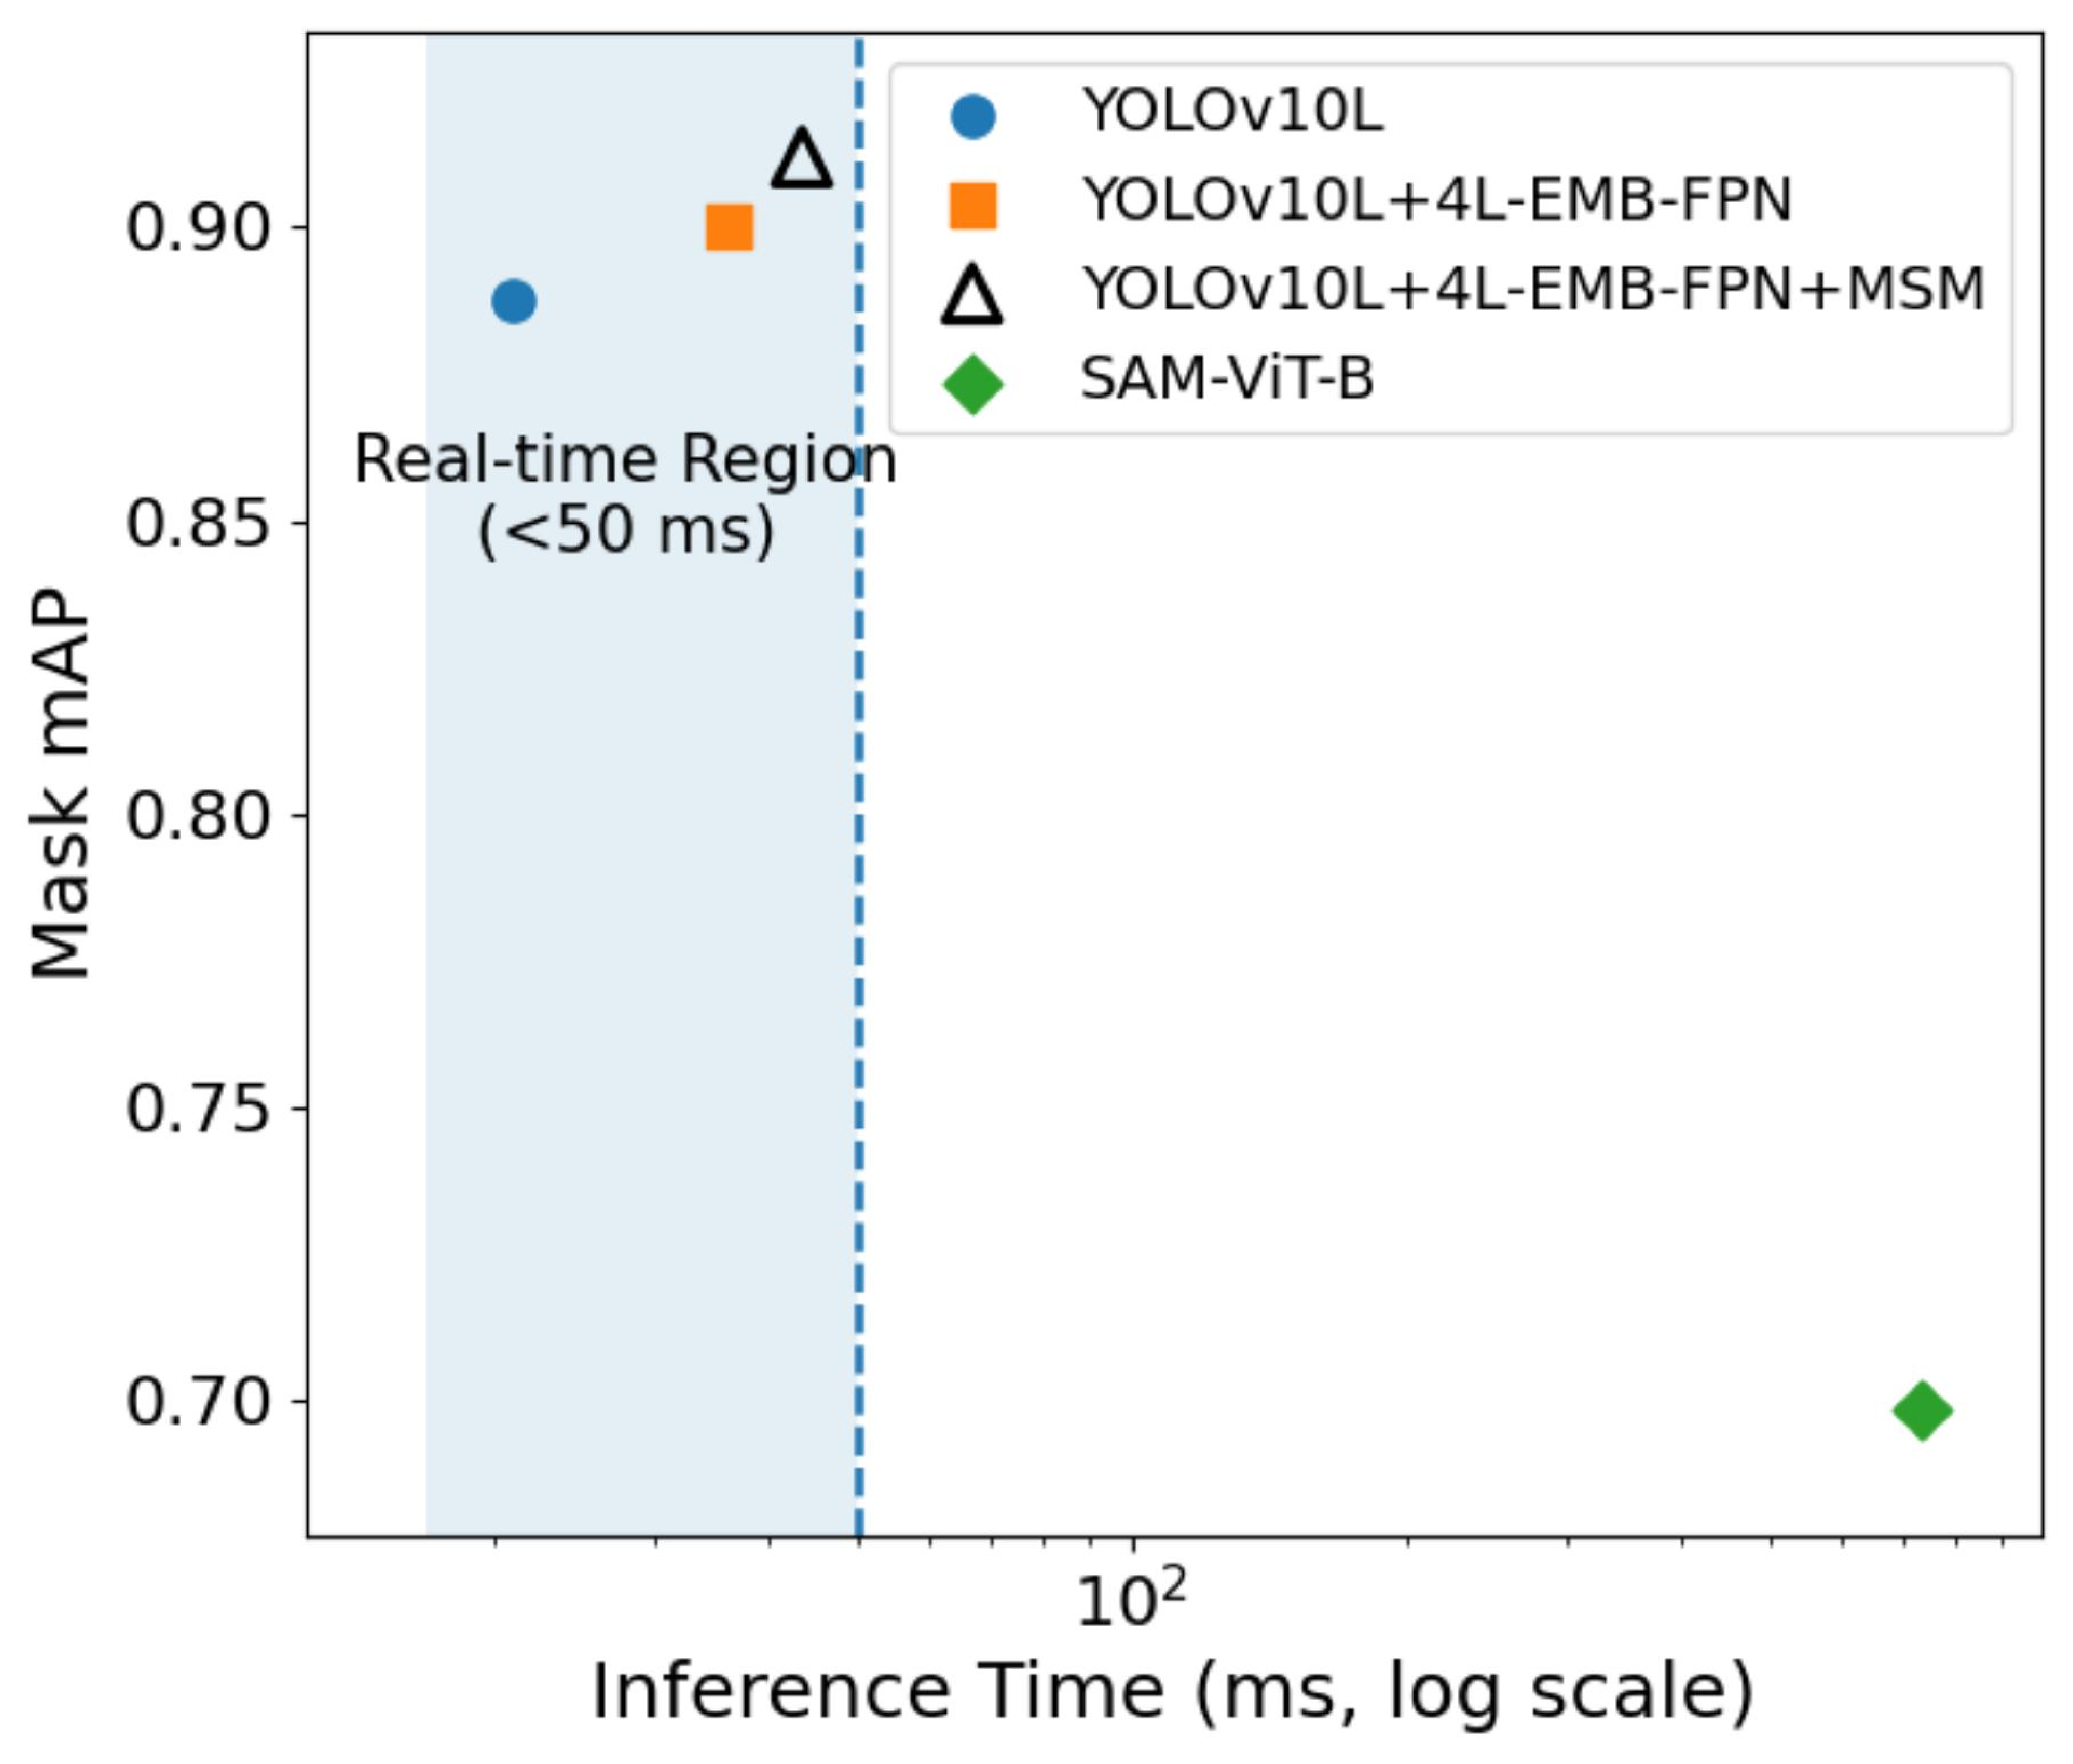
\includegraphics[width=\columnwidth]{figures/fig6.pdf}
\caption{Mask mAP versus inference time for different segmentation models.}
\label{fig:comparison_time}
\end{figure}

The baggage distribution was designed according to airport statistics collected from three airports across eight flights, including 515 items. Suitcases accounted for 94\% of the samples, soft bags for 5\%, and irregular objects for 1\%. More than 90\% of the samples contained strong tag interference. To simulate operational difficulty, random scenarios were generated, including single baggage placement (83\%), two-item contact (10\%), three-item stacking (2\%), and sidewall occlusion (5\%).

For 2D segmentation evaluation, a dataset named SegData was constructed with 49,359 training images and 10,344 testing images captured under different illumination, viewpoints, and distances. For 3D modeling evaluation, OBBData-test was constructed from 1,209 suitcase samples selected from SegData-test. The ground-truth OBBs were manually refined in 3D point clouds. Suitcases were selected because they dominate the baggage distribution and provide stable centroid and yaw references, whereas soft bags are deformable and difficult to annotate consistently.

\subsection{Segmentation Performance}
Three models were trained on SegData-train and evaluated on SegData-test: YOLOv10L, YOLOv10L with 4L-EMB-FPN, and YOLOv10L with both 4L-EMB-FPN and MSM, i.e., MSAM-Net. Table~\ref{tab:seg} reports the quantitative segmentation results.

\begin{table}[!t]
\centering
\caption{Segmentation performance on SegData-test.}
\label{tab:seg}
\begin{tabular}{lcc}
\toprule
Method & Box mAP & Mask mAP \\
\midrule
YOLOv10L & 0.9185 & 0.8877 \\
+ 4L-EMB-FPN & 0.9417 & 0.9004 \\
+ MSM (MSAM-Net) & 0.9524 & 0.9120 \\
\bottomrule
\end{tabular}
\end{table}

The 4L-EMB-FPN improves mask mAP by 1.27\% compared with the YOLOv10L baseline, and the full MSAM-Net further increases the gain to 2.43\%. These results show that enhanced multi-scale aggregation and attention-guided mask refinement improve segmentation quality under tag and strap interference.

Inference latency on the AX650N processor is reported in Table~\ref{tab:latency}. MSAM-Net increases the inference time from 21.1$\mathrm{ms}$ to 43.6$\mathrm{ms}$, but remains below the 50$\mathrm{ms}$ real-time threshold required for 20~Hz conveyor-based manipulation. By comparison, SAM-ViT-B requires 733.6$\mathrm{ms}$ per frame and is therefore unsuitable for embedded real-time deployment in this system (as shown in Fig.~\ref{fig:comparison_time}. SAM was evaluated without task-specific fine-tuning and achieved a mask mAP of 0.69. However, the comparison primarily demonstrates computational feasibility under industrial constraints.

\begin{table}[!t]
\centering
\caption{Inference time comparison on AX650N.}
\label{tab:latency}
\begin{tabular}{lc}
\toprule
Method & Inference time (ms) \\
\midrule
YOLOv10L & 21.1 \\
+ 4L-EMB-FPN & 36.1 \\
+ MSM (MSAM-Net) & 43.6 \\
SAM-ViT-B & 733.6 \\
\bottomrule
\end{tabular}
\end{table}

\begin{figure}[!t]
\centering
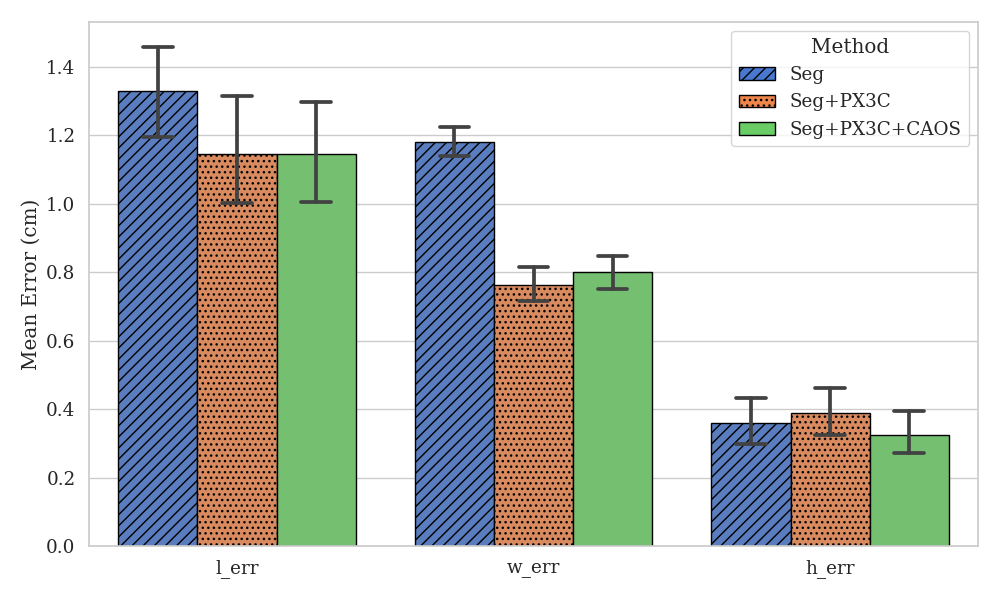
\includegraphics[width=\columnwidth]{figures/fig7.png}
\caption{Comparison of dimension estimation errors before and after PX3C and CAOS. Error bars indicate 95\% confidence intervals.}
\label{fig:estimation}
\end{figure}

\subsection{3D Modeling Accuracy}
To evaluate PX3C and CAOS, dimension and pose estimation errors were computed on OBBData-test. Dimension error was defined as the absolute error in length, width, and height. Pose error included centroid localization error and yaw error in the X--Y plane. Fig.~\ref{fig:estimation} compares dimension estimation before and after PX3C and CAOS, with error bars indicating 95\% confidence intervals.

\begin{figure}[!t]
\centering
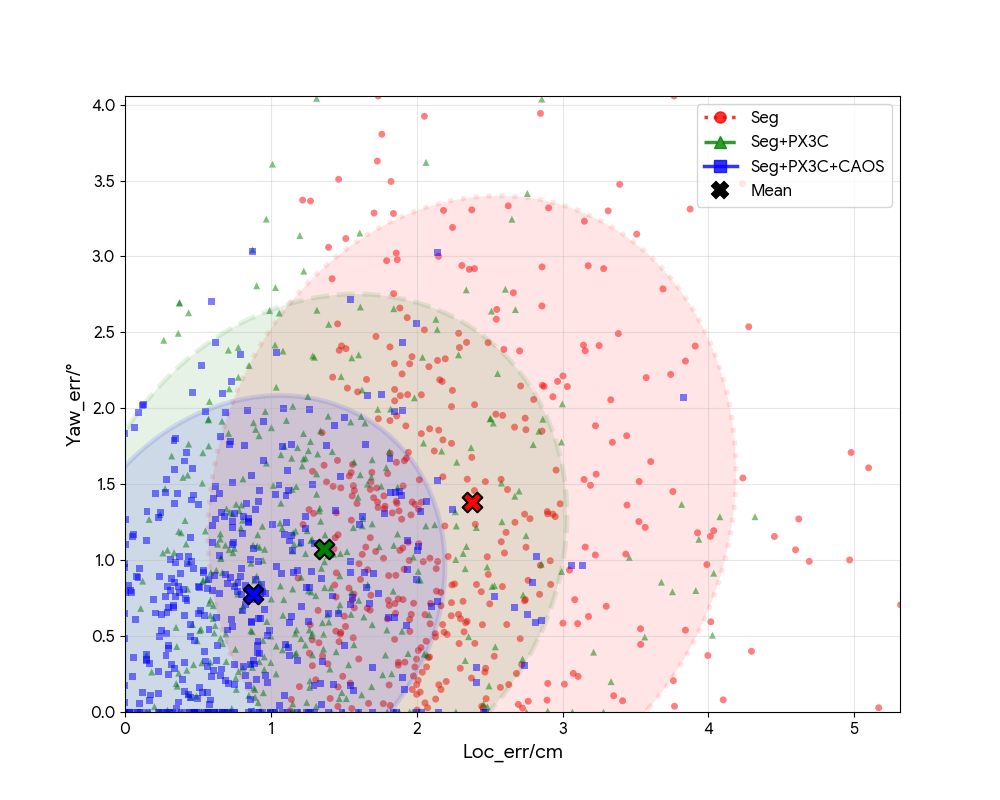
\includegraphics[width=\columnwidth]{figures/fig8.png}
\caption{Localization and yaw error distributions for different modeling stages. Ellipses represent 95\% confidence regions.}
\label{fig:disturbance}
\end{figure}

Compared with segmentation-only modeling, PX3C reduces the width estimation error by 35.5\%. The combined PX3C+CAOS pipeline further stabilizes the estimates. The length estimation error decreases by approximately 13.8\%, and the height estimation error reaches its minimum value of 0.33$\mathrm{cm}$ when both modules are applied. The overall downward shift of the confidence intervals indicates consistent improvement.

The pose-error distributions are shown in Fig.~\ref{fig:disturbance}. Each scatter point corresponds to one sample, and the ellipses denote 95\% confidence regions. Localization error decreases from 2.38$\mathrm{cm}$ using segmentation-only modeling to 1.36$\mathrm{cm}$ with PX3C and to 0.88$\mathrm{cm}$ with CAOS. Yaw error decreases from $1.38^{\circ}$ to $0.78^{\circ}$. These results confirm that PX3C suppresses geometric outliers and CAOS reduces temporal fluctuations.

\begin{figure*}[!t]
\centering
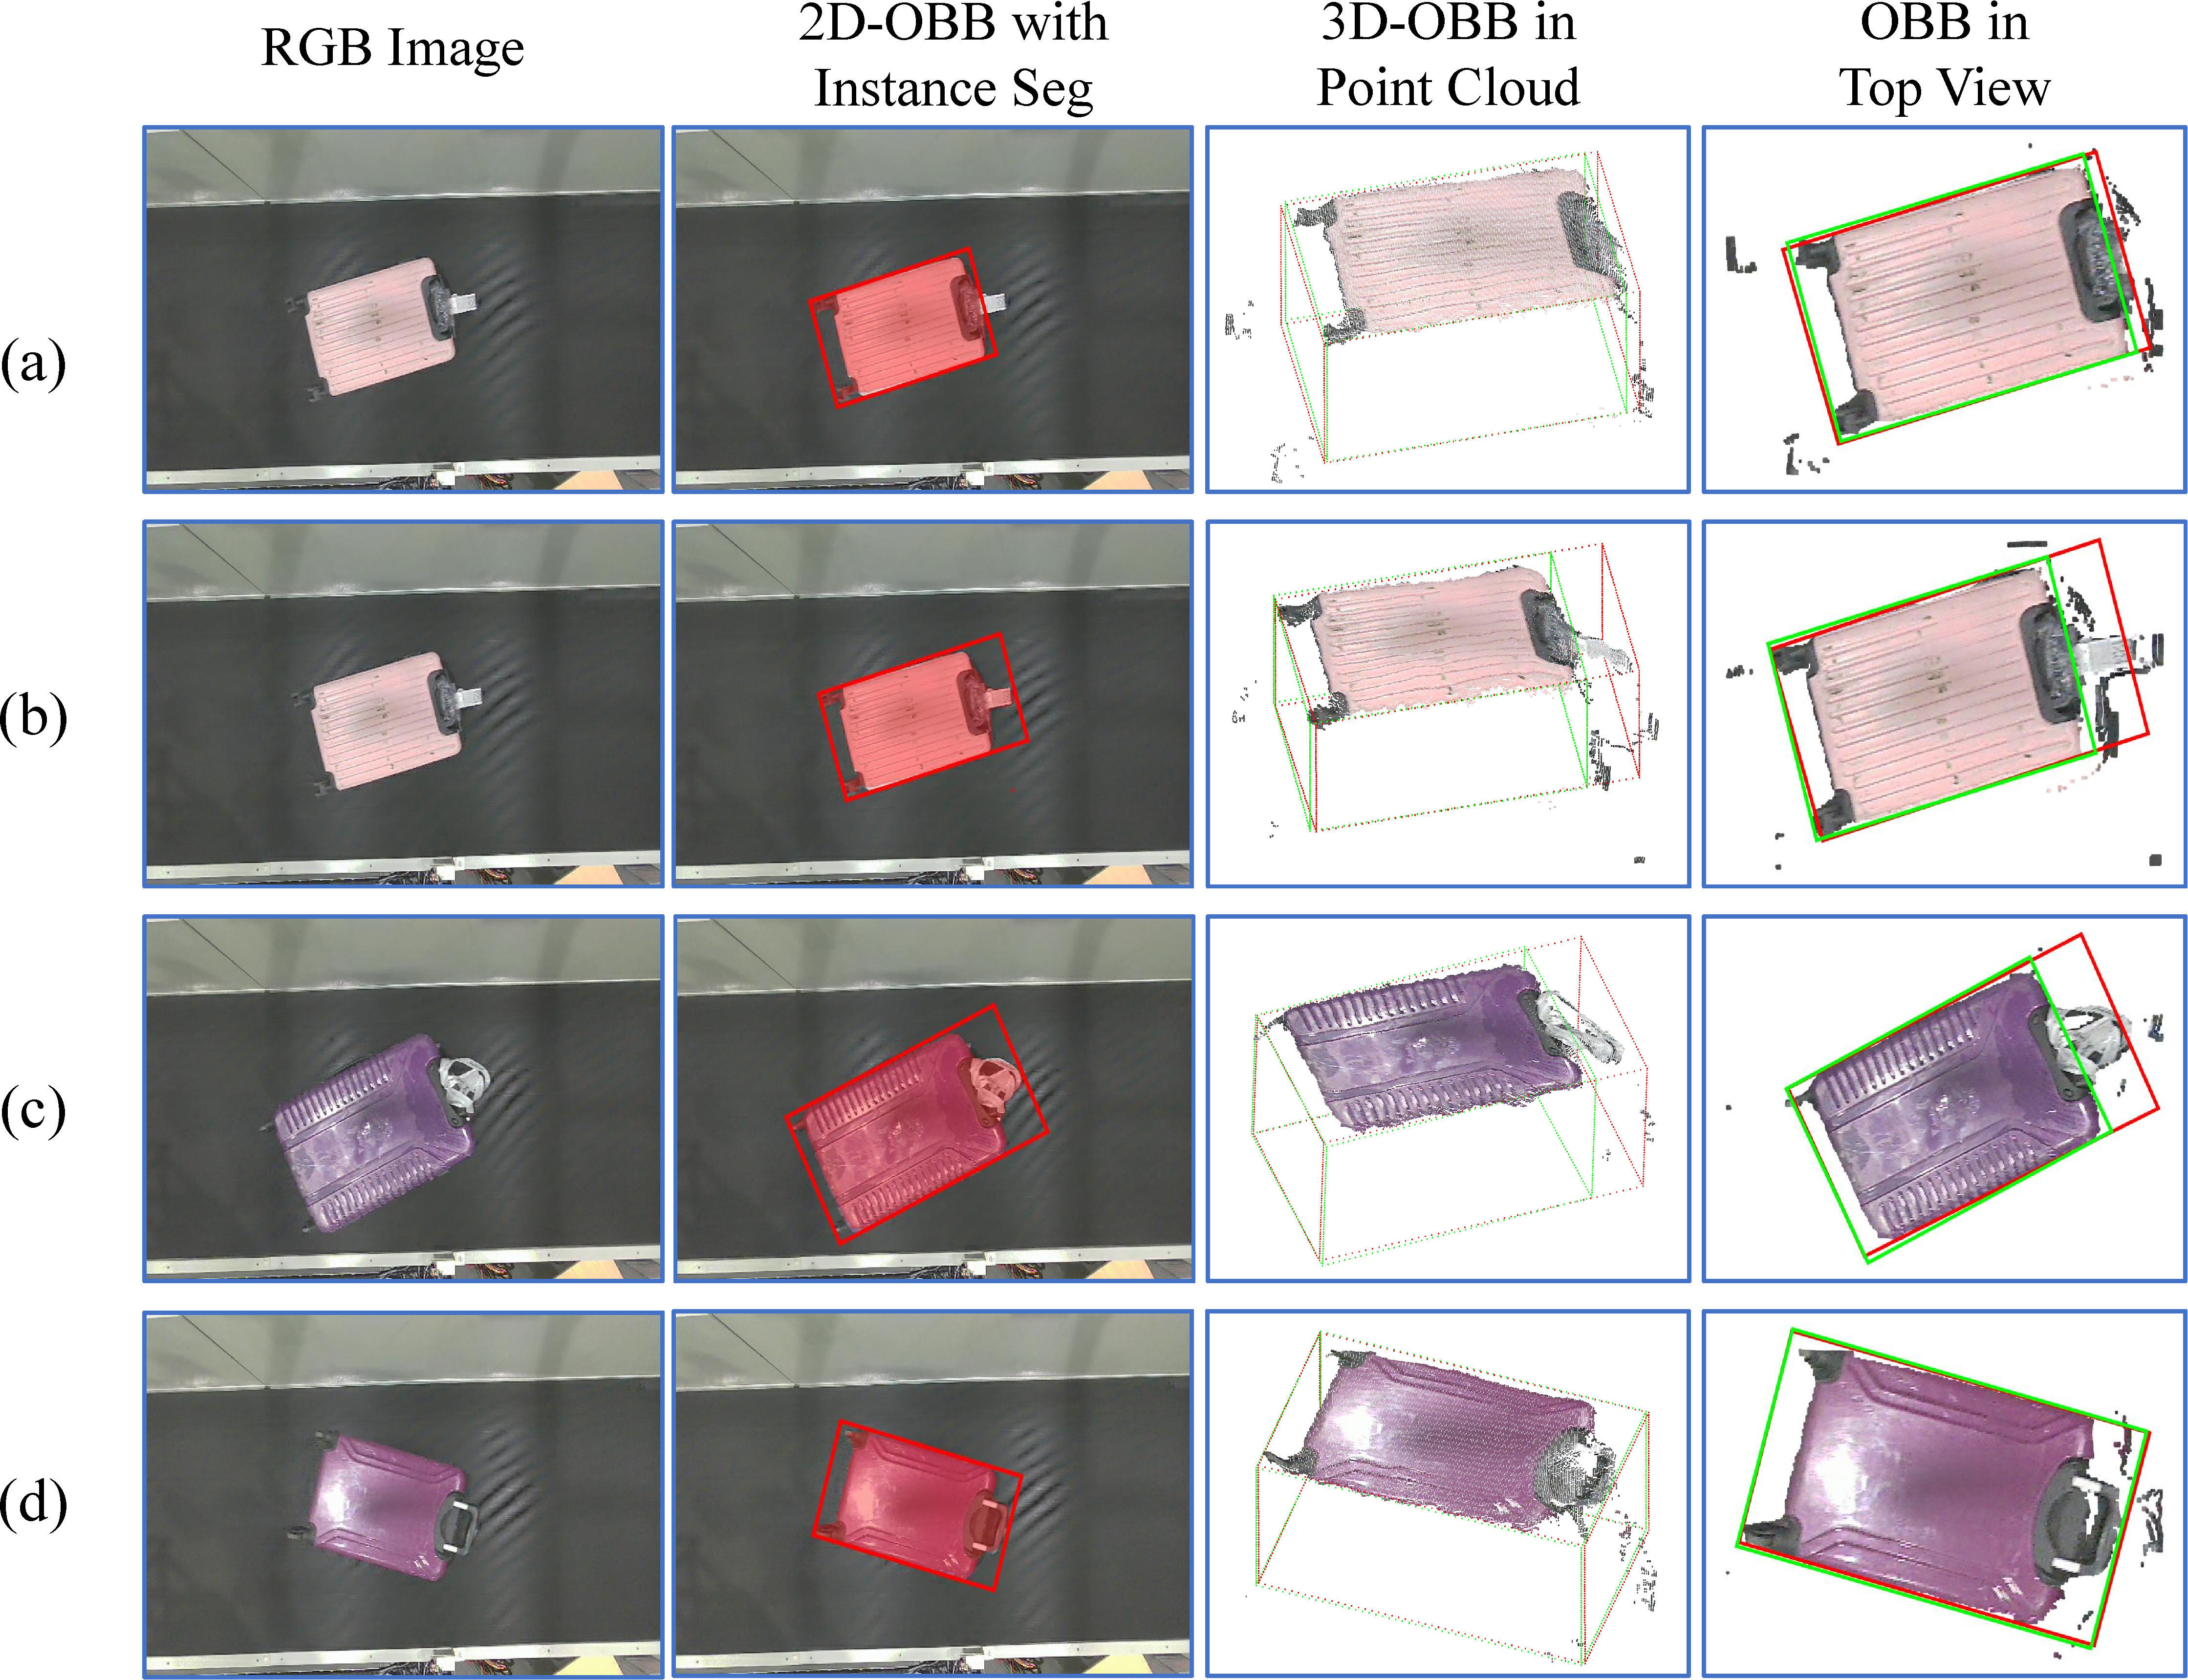
\includegraphics[width=\textwidth]{figures/fig7.pdf}
\caption{Qualitative OBB comparison before and after PX3C filtering.}
\label{fig:represent}
\end{figure*}

Representative qualitative OBB comparisons are shown in Fig.~\ref{fig:represent}. Red boxes denote OBBs derived directly from segmentation, while green boxes denote refined OBBs after PX3C filtering. Flexible tags and ribbons are removed effectively, while rigid components such as handles and wheels are preserved. Temporal stabilization results are shown in Fig.~\ref{fig:temporal}, where CAOS reduces abrupt OBB fluctuations across consecutive frames caused by lighting variation, occlusion, and motion blur.

\begin{figure}[!t]
\centering
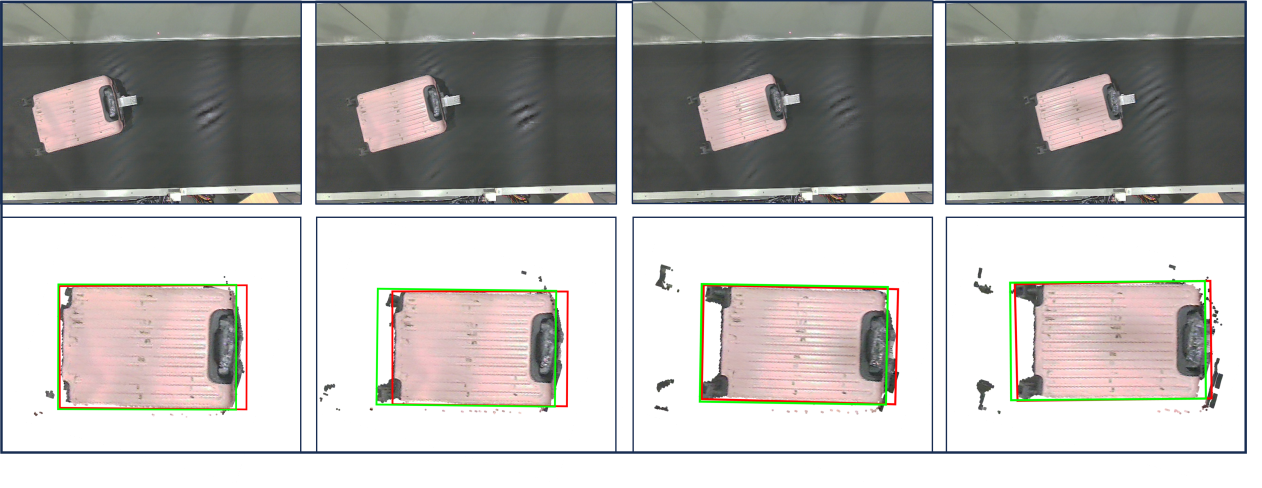
\includegraphics[width=\columnwidth]{figures/fig10.png}
\caption{OBB predictions across consecutive frames with CAOS stabilization.}
\label{fig:temporal}
\end{figure}



\subsection{System-Level Grasping Performance}
Two metrics were used to evaluate system-level performance. General Success Rate (GSR) measures whether the robot successfully lifts the target without dropping it. Precision Success Rate (PSR) requires both a position error below 2$\mathrm{cm}$ and a yaw error below $5^{\circ}$. PSR was computed only for suitcases because they have well-defined geometric references. In multi-object scenarios, the highest object along the Z-axis was selected as the grasping target.

A total of 500 grasping trials were conducted according to the airport baggage distribution, including 470 suitcases, 25 backpacks, and 5 irregular objects. The snapshots are shown in Fig. \ref{fig:snapshot}. An ablation study was performed by incrementally integrating MSAM-Net, PX3C+CAOS, DKF+two-stage planning, and active state regulation. The results are summarized in Table~\ref{tab:ablation}.

\begin{figure*}[!t]
\centering
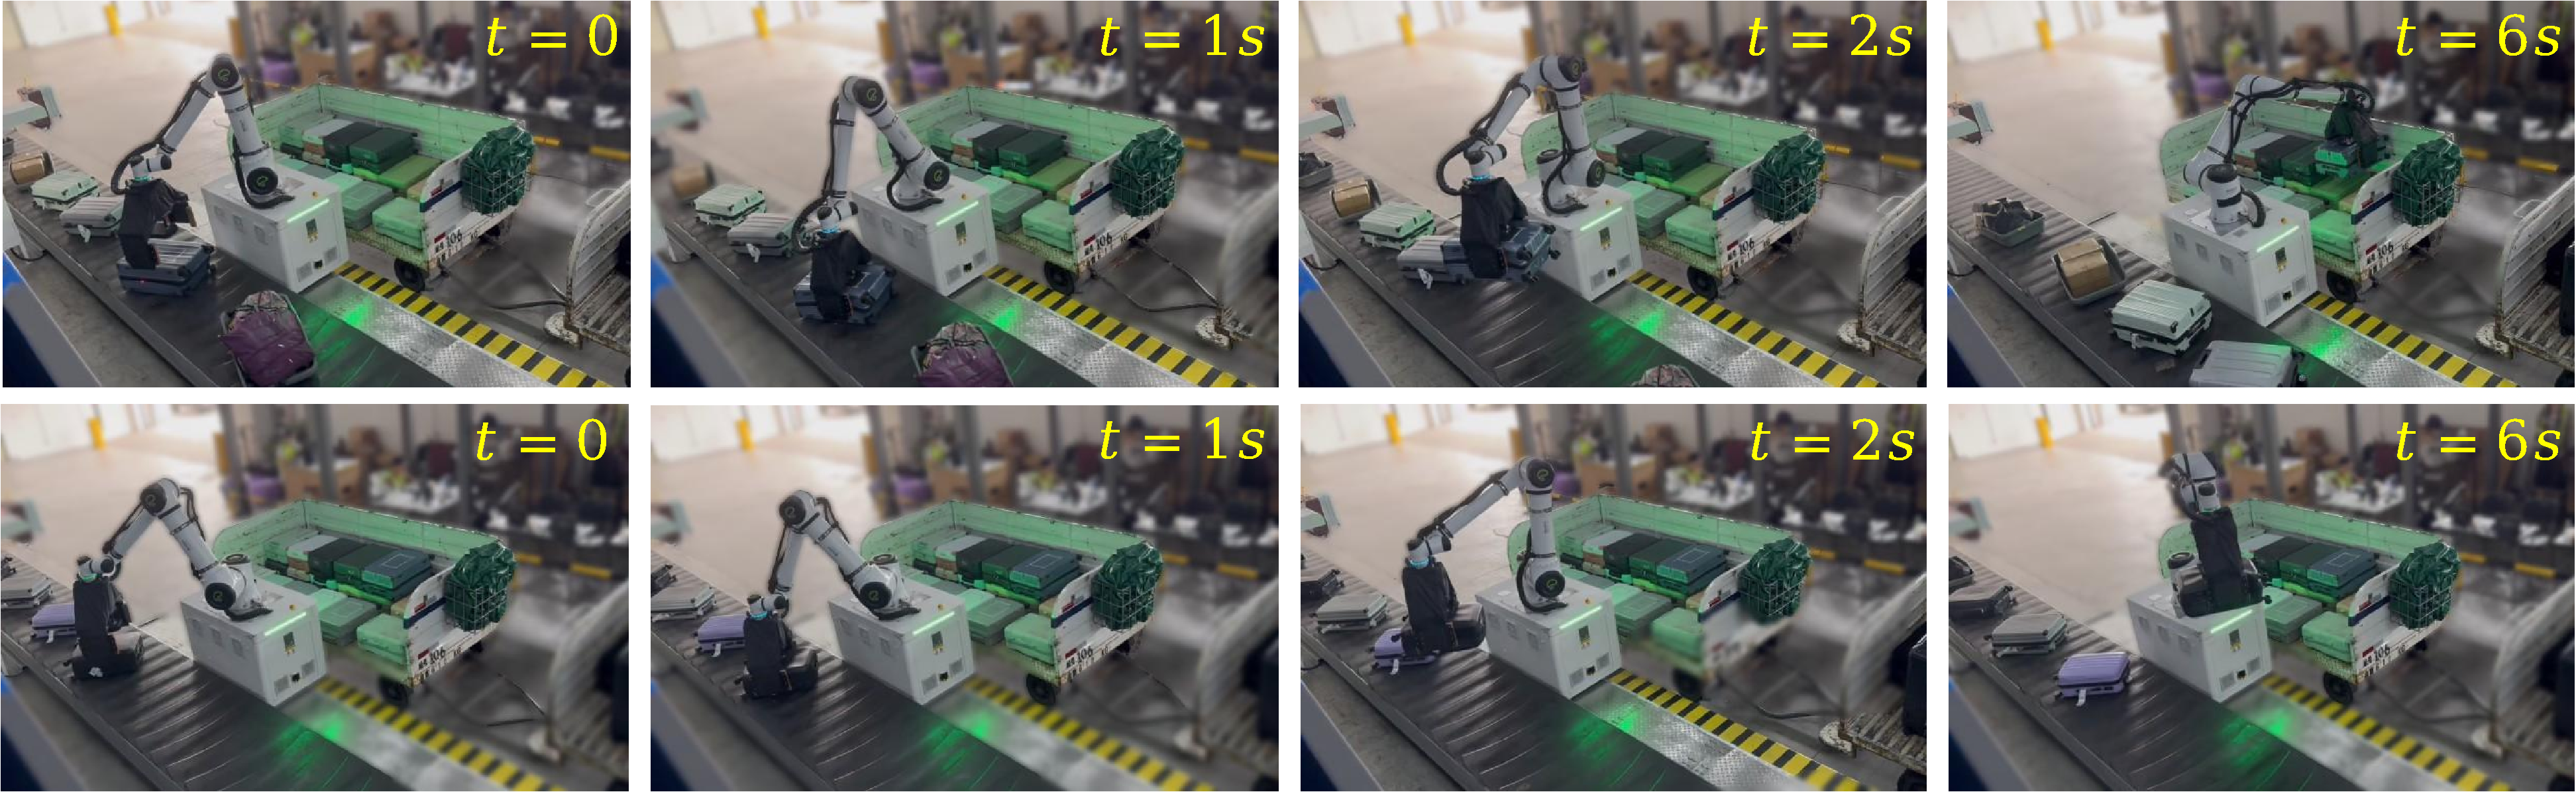
\includegraphics[width=\textwidth]{figures/fig8.pdf}
\caption{Snapshots of the dynamic grasping experiment. The proposed framework achieves robust dynamic grasping on a real conveyor belt in an industrial environment, overcoming the challenges of high-speed motion, cluttered scenes, and control uncertainty.}
\label{fig:snapshot}
\end{figure*}

\begin{table}[!t]
\centering
\caption{Ablation study of different modules on grasping performance.}
\label{tab:ablation}
\begin{tabular}{lcc}
\toprule
Method & GSR (\%) & PSR (\%) \\
\midrule
Baseline (YOLOv10L + PCL) & 93.6 & 62.1 \\
+ Semantic perception (MSAM-Net) & 95.2 & 69.6 \\
+ Geometric consistency (PX3C + CAOS) & 95.6 & 83.8 \\
+ Predictive motion (DKF + two-stage planning) & 96.4 & 84.9 \\
+ Active state regulation (full system) & 96.4 & 92.7 \\
\bottomrule
\end{tabular}
\end{table}

The GSR increases moderately from 93.6\% to 96.4\%, indicating that even the baseline system can lift many objects. In contrast, PSR increases substantially from 62.1\% to 92.7\%. This difference reflects the distinct meanings of the two metrics. GSR primarily measures grasp feasibility, whereas PSR evaluates geometric precision under strict position and orientation constraints. The baseline system can often lift baggage despite moderate pose errors, but inaccurate localization and unstable OBB estimation significantly degrade precise placement. The large PSR improvement demonstrates that the proposed geometric refinement and predictive control modules primarily improve pose accuracy and downstream placement reliability, which are crucial for high-density baggage loading.
\section{Conclusion and Future Work}
This paper presented a closed-loop perception, geometric modeling and control framework for dynamic robotic baggage handling in airport logistics environments. The proposed system tightly integrates semantic perception, geometric consistency modeling, predictive motion planning, and active state regulation. MSAM-Net improves segmentation robustness under severe tag interference through multi-scale aggregation and attention-guided mask refinement. PX3C and CAOS enhance 3D geometric reliability by suppressing residual outliers and stabilizing temporal OBB estimation. The DKF-based predictive motion module and relative-velocity planning strategy enable stable grasp execution under conveyor motion, while active state regulation handles unstable or high-uncertainty configurations.

Experiments on a real robotic platform demonstrate that the proposed framework significantly improves precision-oriented grasping. While the general grasp success rate remains consistently high, the precision success rate improves from 62.1\% to 92.7\%. This gain confirms that accurate geometric modeling and predictive control are essential for industrial deployment where downstream packing efficiency depends on precise pose alignment. Although this work does not explicitly optimize packing policies, it provides the geometric and execution reliability required by high-density loading systems.

Future work will proceed in three directions. First, tactile sensing can be integrated to provide force feedback during grasping, enabling better handling of deformable or visually ambiguous objects. Second, deep reinforcement learning may be used to learn more flexible active-interaction strategies, such as pushing, separating, or reorienting stacked baggage with minimal intervention. Third, high-fidelity simulation and Sim2Real transfer can be used to accelerate data generation and reduce reliance on costly physical experiments. These directions will further improve the autonomy, robustness, and scalability of robotic baggage-handling systems in real airport logistics environments.



\section*{Acknowledgments}
This should be a simple paragraph before the References to thank those individuals and institutions who have supported your work on this article.







%{\appendices
%\section*{Proof of the First Zonklar Equation}
%Appendix one text goes here.
% You can choose not to have a title for an appendix if you want by leaving the argument blank
%\section*{Proof of the Second Zonklar Equation}
%Appendix two text goes here.}



\bibliography{reference}



\bibliographystyle{IEEEtran}








\end{document}


